\chapter{Najkrótsze ścieżki z~jednym źródłem}

W~poprzednim rozdziale omówiliśmy prosty algorytm wyszukiwania najkrótszych ścieżek w~charakterze przykładu na wykorzystanie w~praktyce wcześniej omówionych zagadnień. Doszliśmy do wniosku, że algorytm wykonuje ogromną liczbę operacji, w~tym większość z~nich niepotrzebnie (jak na przykład próby relaksacji krawędzi, wychodzących z~wierzchołków, do których algorytm jeszcze nie potrafił dojść, wykorzystując wcześniej obliczone ścieżki), starając się zminimalizować liczbę tych ostatnich, poprzez wprowadzenie dodatkowych warunków do naszej implementacji. Ich obecność pozwalała mieć nadzieję na efektywniejsze działanie algorytmu, jednak asymptotycznie nie uzyskaliśmy żadnej poprawy, nadal oszacowując czas działania algorytmu na ograniczony przez $O \left( V \cdot E \right)$. Nie umknął też naszej uwadze fakt, iż od kolejności wykonywanych relaksacji głównie zależy liczba operacji, jakie algorytm musi wykonać, aby zwrócić poprawny wynik i~zakończyć pracę. Nic więc dziwnego, że rozwój algorytmiki zaowocował zaproponowaniem wielu innych rozwiązań tego samego problemu, skupiając się przede wszystkim na wymuszeniu takiej kolejności operacji, aby algorytm wykonywał ich jak najmniej.

\section{Sortowanie topologiczne}

Aby przekonać się o~skuteczności takiego podejścia, przedstawimy prosty algorytm \textbf{sortowania topologicznego}, z~którego pomocą będziemy mogli odnaleźć wszystkie najkrótsze ścieżki w~skierowanym grafie ważonym $G = \left( V, E \right)$ w~czasie liniowym (co jest ogromnym skokiem wydajnościowym jeżeli chodzi o~kwadratową złożoność algorytmu Bellmana-Forda)! Niestety, jak się będziemy mieli okazję przekonać, algorytm \textbf{sortowania topologicznego} narzuci nam bardzo silne ograniczenie na postać grafu, dla którego będziemy chcieli dokonywać obliczeń, przez co algorytm ten nie będzie już taki atrakcyjny, jakim wydawał się na początku, by nie powiedzieć~--- bezużyteczny. Warto poświęcić mu jednak trochę uwagi, gdyż stanowi dogodne tło do dalszych rozważań.

\textbf{Sortowanie topologiczne} polega na takim posortowaniu wierzchołków, aby dla każdej pary $ \left( v_{i}, v_{j} \right)$, w~przypadku istnienia krawędzi pomiędzy tymi wierzchołkami, prowadzącej z~$v_{i}$ do $v_{j}$, w~już posortowanym ciągu $v_{i}$ znajdował się przed wierzchołkiem, do którego dana krawędź prowadzi. Innymi słowy sortowanie topologiczne prowadzi do ustalenia możliwej kolejności odwiedzeń wszystkich wierzchołków w~grafie. Jako przykład w~literaturze najczęściej można spotkać problem stworzenia listy kolejno wykonywanych czynności na podstawie posiadanego grafu, przedstawiającego zależności między poszczególnymi czynnościami (na przykładzie pieczenia ciasta, bądź kolejności zakładania ubrań)~\cite[$22.4$]{Cormen}. 

Mówiąc o~kolejności w~grafie oczywistym więc jest, że nie uda nam się ustalić odpowiedniego porządku dla grafów, które będą zawierały cykle. Poniżej przedstawimy dwie popularne metody wyznaczania takiego porządku, gdzie pierwsza z~nich okaże całkowicie bezradna w~obliczu wystąpienia cyklu, zaś druga będzie je po prostu ignorować. Należy wyraźnie podkreślić, że w~tym drugim przypadku dla grafu zawierającego cykle jako wynik nie otrzymamy porządku topologicznego, tak więc będzie on~--- z naszego punktu widzenia~--- bezwartościowy.

\subsection{Algorytm Khana}

Jednym z~naturalnych sposobów na wyznaczenie, opisanej przez nas, kolejności wierzchołków jest rozpoczęcie ich spisywania od tych, do których nie prowadzą żadne krawędzie~--- powiedzmy, że takie wierzchołki nie mają żadnych ,,wymagań'' by mogły być odwiedzone. Skoro odwiedziliśmy już wszystkie takie wierzchołki, możemy założyć, że pewne ,,wymagania'', które te wierzchołki sobą reprezentują, zostały spełnione i~posiadamy nieco większe ,,możliwości'', by czynić zadość ,,wymaganiom'' pozostałych wierzchołków. Takie rozumowanie, przeprowadzone dla wszystkich wierzchołków w~grafie bez cykli da nam listę, na którą zostały spisane wierzchołki w~porządku topologicznym. Łatwo sobie wyobrazić analogiczne rozumowanie w~przypadku wystąpienia cyklu: gdy wierzchołek $v_{A}$ na swojej ,,liście wymagań'' posiada takie, by przed jego odwiedzeniem był odwiedzony węzeł $v_{B}$ (co przedstawilibyśmy na grafie w~postaci krawędzi z~$v_{B}$ do $v_{A}$) a~wierzchołek $v_{B}$~--- by przed jego odwiedzeniem był odwiedzony węzeł $v_{A}$. Widzimy, że żadnego z~tych warunków nie da się spełnić. Algorytm, opisujący takie działanie, wyglądać mógłby następująco:

\begin{pseudokod}[!htbp]
\DontPrintSemicolon
\KwIn{Graf $G = \left( V, E\right)$.}
\KwResult{Lista $O$ z~posortowanymi topologicznie wierzchołkami.}
\Begin{
	$ S \longleftarrow $ zbiór wszystkich wierzchołków, do których nie prowadzą żadne krawędzie \;
	$ O \longleftarrow \emptyset $ \;
	\While{$S$ nie jest pusta}{
		Przepnij wierzchołek $v_{i}$ z~$S$ na koniec listy $O$ \;
		\ForEach{$e_{ij} : v_{i} \overset{1} \leadsto v_{j}$}{
			Usuń krawędź $e_{ij}$ z~grafu $G$ \;
			\If{ do $v_{j}$ nie wchodzą już żadne krawędzie } {
				Wstaw wierzchołek $v_{j}$ do $S$ \;
			}
		}
	}
	\eIf{ w~grafie $G$ nadal są wierzchołki }{
		\Return \KwNull \;
	}{
		\Return $O$ \;
	}
}
\caption{ KHAN-TOPOLOGICAL-SORT $\left( G \right)$\label{alg:KhanTopologicalSort}}
\end{pseudokod}

Algorytm działa niemal identycznie jak w~przeprowadzonym przez nas rozumowaniu. Za punkt wejścia obieramy listę wierzchołków, do których nie prowadzą żadne krawędzie, zaś przez cały czas trwania algorytmu usuwamy wszystkie te, które wychodzą od wierzchołków już odwiedzonych. W~momencie, gdy do jakiegoś węzła przestają prowadzić krawędzie w~grafie, dodajemy go do listy węzłów, które sekwencyjnie odwiedzamy. Jest to sytuacja równoważna ze spełnieniem wszystkich ,,wymagań'', by dany wierzchołek móc odwiedzić. Co może okazać się problematyczne, to zdobycie informacji na temat liczby krawędzi, wchodzących do każdego pojedynczego wierzchołka, gdyż~--- jak pamiętamy~--- zdecydowaliśmy się na przedstawienie struktury połączeń w~grafie za pomocą list sąsiedztwa, które nam takiej wiedzy nie dają. Problem jest jednak bardzo prosty do rozwiązania~--  aby takie informacje zdobyć, musimy przejść po wszystkich krawędziach w~grafie, gromadząc w~osobnej tablicy $deg \left[1 \cdots \left| V \right| \right]$ informację o~liczbie łuków, wchodzących do poszczególnych węzłów, o~identyfikatorach z~zakresu od $1$ do $\left| V \right|$ (przy czym nie interesuje nas nic poza ich liczebnością, zaś czas, jaki potrzebujemy na jednorazowe przejście po wszystkich krawędziach grafu $G$, jest oczywiście liniowy w odniesieniu do ich liczby). Następnie ta tablica posłuży nam do symulowania takich wydarzeń jak: usunięcie krawędzi z~grafu, sprawdzenie czy do danego wierzchołka przestały prowadzić jakiekolwiek łuki. Nie usuwając krawędzi z~grafu zaraz po przejściu przez nie a~jedynie symulując ich usunięcia, narażamy się na sytuacje, w~których algorytm zacznie nieprzerwanie krążyć pomiędzy węzłami w~grafie, które tworzą cykl~--- sprawdzenie, czy taki występuje, następuje dopiero pod sam koniec algorytmu w~wierszach $9$--$12$. Możemy sobie jednak z~tym problemem poradzić równie łatwo, co z~wyznaczaniem liczby węzłów wchodzących do grafu. Jedyne, co musimy zauważyć to fakt, że z~każdym powtórzeniem instrukcji $3$--$8$ dodajemy do zbioru $S$ kolejny wierzchołek grafu. W~przypadku natrafienia na cykl i~nieusuwania krawędzi, każde wejście do węzła $v_{i}$ po ścieżce, należącej do cyklu, spowoduje, że zmniejszymy wartość licznika $deg \left[ i \right]$ o~jeden (symulując tym samym usunięcie krawędzi). Jeżeli okaże się, że po pierwszym przejściu taką ścieżką $deg \left[ i \right] = 0 $ (co odpowiada braku krawędzi wchodzących do $v_{i}$) dla każdego węzła, należącego do cyklu, to wpadniemy w~nieskończoną pętlę, dodając do zbioru $S$ kolejne węzły, usuwając je z powrotem nieco dalej (w~kroku $4$). Jednym z~wielu pomysłów na rozwiązanie tego problemu jest wprowadzenie ograniczenia na liczbę elementów listy $O$~--- dla poprawnie wykonanego algorytmu będzie ona zawsze długości $ \left| V \right| $, podczas gdy dla omawianego przypadku złego zachowania się algorytmu bardzo szybko liczba tych elementów przekroczy ich oczekiwaną liczbę.

\begin{figure}[!htbp]
	\centering
	\begin{subfigure}[b]{0.25\textwidth}
		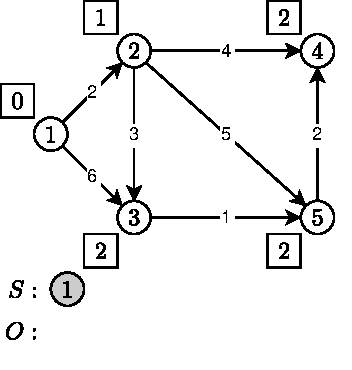
\includegraphics[width=\textwidth]{Chapter_II/KHAN-TOPOLOGICAL-SORT-Example/a.pdf}
		\caption{}
	\end{subfigure}%
	\qquad
	\begin{subfigure}[b]{0.25\textwidth}
		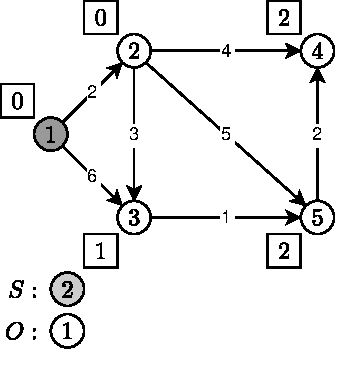
\includegraphics[width=\textwidth]{Chapter_II/KHAN-TOPOLOGICAL-SORT-Example/b.pdf}
		\caption{}
	\end{subfigure}
	\qquad
	\begin{subfigure}[b]{0.25\textwidth}
		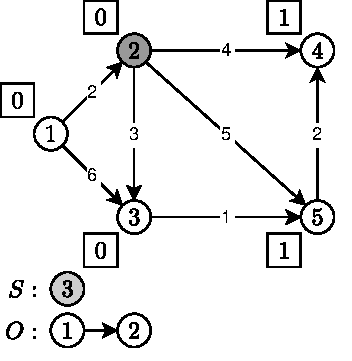
\includegraphics[width=\textwidth]{Chapter_II/KHAN-TOPOLOGICAL-SORT-Example/c.pdf}
		\caption{}
	\end{subfigure}
	\begin{subfigure}[b]{0.25\textwidth}
		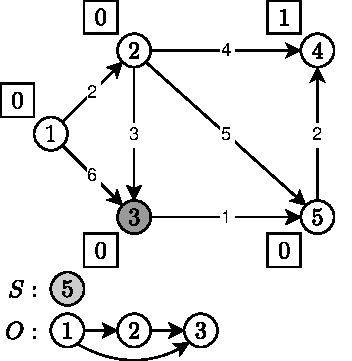
\includegraphics[width=\textwidth]{Chapter_II/KHAN-TOPOLOGICAL-SORT-Example/d.pdf}
		\caption{}
	\end{subfigure}%
	\qquad
	\begin{subfigure}[b]{0.25\textwidth}
		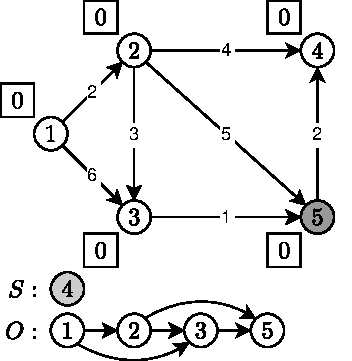
\includegraphics[width=\textwidth]{Chapter_II/KHAN-TOPOLOGICAL-SORT-Example/e.pdf}
		\caption{}
	\end{subfigure}
	\qquad
	\begin{subfigure}[b]{0.25\textwidth}
		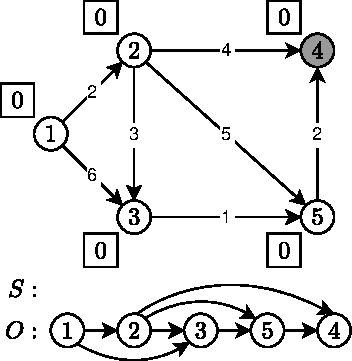
\includegraphics[width=\textwidth]{Chapter_II/KHAN-TOPOLOGICAL-SORT-Example/f.pdf}
		\caption{}
	\end{subfigure}
	\caption{\textbf{Działanie algorytmu Khana} \textbf{(a)} Sytuacja początkowa algorytmu. Na liście $S$ znajdują się wszystkie węzły, do których~--- przed rozpoczęciem działania algorytmu~--- nie wchodziły żadne krawędzie. Przy każdym z~węzłów (w kwadratach) znajduje się liczba takich krawędzi $e \in E$, które wchodzą do danego wierzchołka~--- reprezentują one elementy tablicy $deg \left[ i \right]$, gdzie $i$ to identyfikator węzła, przy którym znajduje się dany element. \textbf{(b)} Algorytm wybiera z~listy $S$ jedyny możliwy element i~usuwa z~grafu wszystkie krawędzie, wychodzące z~wybranego węzła, dodając jednocześnie do listy $O$ każdy węzeł, do którego, w~wyniku usunięcia tych krawędzi, nie prowadzi już żaden łuk. Usuwanie połączenia $v_{i} \overset{1} \leadsto v_{j}$ symbolizujemy zmniejszeniem wartości elementu $deg \left[ j \right]$. \textbf{(c)} Usunięcie krawędzi wychodzących z~następnego, pobranego z~listy $S$ elementu, spowodowało dodanie do niej wierzchołka $v_{3}$. Badany element $v_{2}$~--- podobnie jak w~poprzednim przypadku~--- po wyciągnięciu z~listy $S$, przepinamy do listy $O$. \textbf{(d)} Dodanie do listy $S$ węzła $v_{5}$ w wyniku usunięcia wszystkich krawędzi $e \in \left\{ e_{ij} : i~= 3 \right\}$. Przepięcie badanego elementu $v_{3}$ na listę $O$. \textbf{(e)} Wykonanie kolejnej pętli algorytmu i~dodanie skanowanego elementu $v_{5}$ do listy wynikowej.  \textbf{(f)} Ostatni krok algorytmu. Zauważmy, że w~grafie nie ma już żadnych łuków (wszystkie elementy z~tablicy $deg$ zostały wyzerowane), więc algorytm zakończył się poprawnie~--- badana sieć nie miała cykli.} \label{fig:exampleKhan}
\end{figure}

Czas działania takiej metody jest oczywiście liniowy, zależny od liczby zarówno węzłów, jak i~krawędzi w~grafie. Zależnie od tego, czy w~węzłach przechowujemy informację o~liczbie wchodzących do nich krawędzi, te pierwsze będziemy musieli przejrzeć w~czasie $O \left( \left| V \right| \right)$ w~poszukiwaniu takich węzłów, które takowych krawędzi nie mają, zaś jeżeli takich informacji nie mamy~--- wówczas będziemy musieli je sami wygenerować, skanując wszystkie krawędzie w~grafie (co zajmie nam $O \left( \left| E \right| \right)$ czasu). Bez względu na wcześniej wykonany krok, właściwa część algorytmu polega na usunięciu wszystkich krawędzi z~grafu (gdyż taki chcemy uzyskać rezultat dla prawidłowej sieci) w~czasie $O \left( \left| E \right| \right)$.

\subsection{Przeszukiwanie w~głąb}

Alternatywnym sposobem na topologiczne uporządkowanie grafów w~sieci jest wykorzystanie właściwości, posiadanych przez prosty algorytm przeszukiwania w~głąb, w~skrócie \textsf{DFS} (ang. \textit{Depth-First Search}). Aby posortować topologicznie wszystkie węzły w~gafie $G = \left( V, E \right)$, wykorzystujemy fakt, że wspomniany algorytm oznacza dany węzeł $v$ jako przetworzony dopiero w~momencie, gdy wszystkie węzły, do których jest w~stanie dojść z~badanego węzła, są oznaczone. Innymi słowy nie jest możliwa sytuacja, by w~grafie został oznaczony węzeł, którego wszystkie dzieci (a także jego dalsi potomkowie) nie zostały oznaczone. Zapisując kolejność takich operacji (oznaczania węzłów jako przetworzone) a~następnie odtwarzając ją w~kolejności odwrotnej, uzyskujemy listę z~poprawnie posortowanymi topologicznie węzłami (odwrotna sytuacja do przedstawionej wcześniej ma następującą interpretacje: żaden węzeł $v_{i}$ nie zostanie zaznaczony, gdy istnieje jakikolwiek węzeł $v_{j}$, który jest jeszcze nie zaznaczony, a~który posiada krawędź $v_{j} \overset{1} \leadsto v_{i}$).

\begin{pseudokod}[!htbp]
\DontPrintSemicolon
\KwIn{Graf $G = \left( V, E\right)$.}
\KwResult{Lista $O$ z~posortowanymi topologicznie wierzchołkami.}
\Begin{
	Wykonaj \textsf{DFS} dla grafu wejściowego $G$ \;
	Wstaw na początek listy $O$ każdy wierzchołek $v$, kiedy ten tylko zostanie oznaczony jako przetworzony. \;
	\Return $O$ \;
}
\caption{ BFS-TOPOLOGICAL-SORT $\left( G \right)$\label{alg:BFSTopologicalSort}}
\end{pseudokod}

W algorytmie niejawnie dokonujemy odwrócenia elementów, które znajdują się na liście $O$, poprzez wstawianie każdego wierzchołka na początek tej listy, nie na jej koniec. Algorytm oczywiście działa w~czasie liniowym, podobnie jak sam \textsf{DFS} ($ \Theta \left( \left| V \right| + \left| E \right| \right)$). Wspomnieliśmy na początku rozdziału, że drugi z~omawianych algorytmów posiada nad pierwszym tę przewagę, że nie przerywa pracy nawet w~momencie napotkania cyklu. Nie jest to do końca prawdą, gdyż zachowanie się algorytmu \textsf{DFS} głównie zależy od intencji jego autora, lecz możemy napisać go w~taki sposób, aby podczas przeglądania grafu wgłąb, po natrafieniu na wierzchołek, który został już odwiedzony, algorytm kontynuował swoją pracę (to jest albo wycofał się z~aktualnie badanego wierzchołka, zaznaczając go jako przetworzony, albo~--- w~przypadku, gdy pozostałe krawędzie badanego węzła prowadzą do jeszcze nieodwiedzonych węzłów~--- kontynuował przeszukiwanie wgłąb). Innymi słowy~--- możemy go zmusić by ignorował cykle, występujące w~badanym grafie.

\begin{figure}[!htbp]
	\centering
	\begin{subfigure}[b]{0.2\textwidth}
		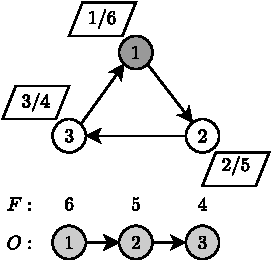
\includegraphics[width=\textwidth]{Chapter_II/BFS-TOPOLOGICAL-SORT-Example/a.pdf}
		\caption{}
	\end{subfigure}%
	\qquad \qquad
	\begin{subfigure}[b]{0.18\textwidth}
		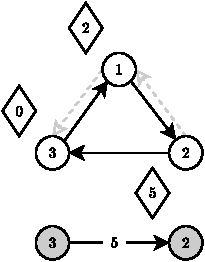
\includegraphics[width=\textwidth]{Chapter_II/BFS-TOPOLOGICAL-SORT-Example/b.pdf}
		\caption{}
	\end{subfigure}
	\qquad \qquad
	\begin{subfigure}[b]{0.18\textwidth}
		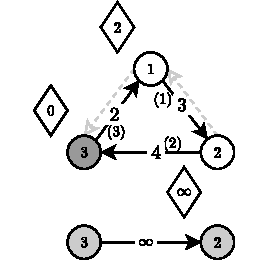
\includegraphics[width=\textwidth]{Chapter_II/BFS-TOPOLOGICAL-SORT-Example/c.pdf}
		\caption{}
	\end{subfigure}
	\caption{\textbf{Przykład złego działania \textsf{DFS} dla grafu z~cyklem} \textbf{(a)} Graf po wykonaniu algorytmu \textsf{DFS}. W~rombach znajdują się charakterystyczne dla grafu wartości w~postaci $x/y$, gdzie $x$ oznacza czas odwiedzenia danego węzła, zaś $y$ to czas jego przetworzenia (po przetworzeniu wszystkich jego dzieci i~ich potomków oraz wycofaniu się z~niego). Lista $O$ zawiera ,,poprawnie'' uporządkowane węzły, w~kolejności malejącej względem czasu przetwarzania węzłów. Algorytm rozpoczyna pracę od pierwszego węzła w~grafie. \textbf{(b)} Poprawnie wykonany algorytm wyszukiwania najkrótszej ścieżki $v_{3} \overset{1} \leadsto v_{2}$~--- $c \left( 3, 2 \right) = \delta \left( 3, 2 \right) = 5$. \textbf{(c)} Błędne rozwiązanie dla algorytmu opartego o~listę $O$ z~rysunku pierwszego. Cyfry w~nawiasach oznaczają kolejność wykonywania relaksacji, wynikającej z~uporządkowania węzłów na liście $O$.} \label{fig:exampleDFS}
\end{figure}

Niestety~--- choć początkowo może się wydawać, że ignorowanie cykli nie szkodzi, a~wręcz jest po naszej myśli (algorytm \textsf{DFS}, napotykając ścieżkę, która zamyka cykl, nie zdecyduje się na pójście tą ścieżką, podobnie jak relaksacja takiej ścieżki nigdy nie przyniesie żadnego rezultatu~--- innymi słowy jest zbędna), lecz prosty przykład wystarcza, by algorytm wyszukiwania najkrótszych ścieżek, który opiera się o~sortowanie topologiczne, zwracał nam niepoprawne wyniki dla tak zadanego grafu.

\subsection{Sortowanie topologiczne}

Jak widzimy z~powyższych przykładów, możliwości wykorzystania sortowania topologicznego w~algorytmach wyszukiwania najkrótszych ścieżek są ograniczone jedynie do małej klasy grafów~--- stanowczo za małej, jeżeli chodzi o~grafy reprezentujące rzeczywiste sieci drogowe. Istnieją jednak pewne problemy (mniej trywialne od pieczenia ciasta, czy kolejności nakładania ubrań), w~których taki algorytm się przydaje i~jest chętnie stosowany głównie ze względu na swoją szybkość działania~--- liniową, proporcjonalnie do liczby krawędzi w~grafie \footnote{Szeregowanie zadań, ustalanie zależności pakietów w systemach operacyjnych, itd.}. Implementacja algorytmu sprowadza się do wykonania relaksacji dla wszystkich krawędzi, wychodzących z~węzłów posortowanych topologicznie, w~której to kolejności powinniśmy postępować.

\begin{pseudokod}[!htbp]
\DontPrintSemicolon
\Begin{
	\ForEach{ $v_{i}$ w~porządku topologicznym } {
		\ForEach{$e_{ij} : v_{i} \overset{1} \leadsto v_{j}$}{
			$RELAX \left( v_{i}, v_{j} \right)$ \;
		}
	}
}
\caption{ TOPOLOGICAL-SHORTEST-PATH $\left( G \right)$\label{alg:topologicalShorestPath}}
\end{pseudokod}

Aby udowodnić poprawność działania takiego algorytmu, odwołamy się do dwóch wcześniej przedstawionych lematów: o~optymalnej podstrukturze grafu (\ref{lem:optimalSubstructure}) oraz zbieżności najkrótszych ścieżek (\ref{lem:convergenceProperty}).

\begin{proof}
Załóżmy indukcyjnie, że algorytm przeskanował już wierzchołki $v_{i} : i \in \left\{ 1, 2, \cdots, k \right\}$ i~dla każdego z~nich ich waga jest optymalna ($d \left( i \right) = \delta \left( s, v_{i} \right)$). W~oczywisty sposób pierwszy krok indukcyjny jest spełniony: dla $k = 1$ naszym jedynym wierzchołkiem, który został obsłużony, jest wierzchołek początkowy~--- źródło, którego $d \left( s \right) = \delta \left( s, s \right) = 0$. Przyjrzyjmy się teraz sytuacji, w~której algorytm bada węzeł $\left(k+1\right)$'y (nie $v_{k+1}$). Niech najkrótszą ścieżką do tego węzła będzie $P = \left \langle v_{1}, v_{2}, \ldots, v_{h}, k+1 \right \rangle $. Z~lematu \ref{lem:optimalSubstructure} (o optymalnej podstrukturze) wiemy, że każda podścieżka ścieżki $P$ jest najkrótszą ścieżką (w~szczególności jest nią ścieżka $P^{'} = \left \langle v_{1}, v_{2}, \ldots, v_{h} \right \rangle $). Z~faktu, że wszystkie wierzchołki w~grafie są posortowane topologicznie oraz, że krawędź $v_{h} \overset{1}\leadsto k+1 \in E$ (co nam gwarantuje istnienie ścieżki $P$) wynika, że wierzchołek $v_{h}$ jest węzłem, dla którego $h \in \left\{ 1, 2, \cdots, k \right\}$~--- w~związku z~tym, na mocy założenia indukcyjnego, wartość $v_{h}.d = \delta \left( s, v_{h} \right)$. Zgodnie z~lematem \ref{lem:convergenceProperty}, jeżeli w~dowolnym momencie przed relaksacją krawędzi $v_{h} \overset{1}\leadsto k+1$ wartość $v_{h}.d = \delta \left( s, v_{h} \right)$, to po relaksacji tej krawędzi już zawsze $ \left( k+1 \right).d = \delta \left( s, k+1 \right) $ (jest optymalna). Z~faktu istnienia takiej krawędzi oraz z~uporządkowania topologicznego wszystkich węzłów w~grafie wiemy, że waga, jaką posiada wierzchołek $v_{h}$, zawsze będzie optymalna przed przystąpieniem do przechodzenia po krawędzi $v_{h} \overset{1}\leadsto k+1$, co kończy dowód.\footnote{Przeprowadzając dowód oparliśmy się na rozumowaniu przedstawionym w \cite[$4.4$]{Ahuja:1993:NFT:137406}}
\end{proof}


\begin{figure}[!htbp]
	\centering
	\begin{subfigure}[b]{0.18\textwidth}
		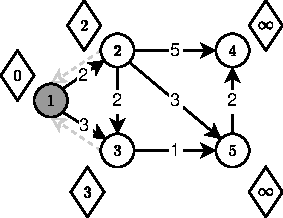
\includegraphics[width=\textwidth]{Chapter_II/TOPOLOGIC-SHORTEST-PATH-Example/a.pdf}
		\caption{}
	\end{subfigure}
	\begin{subfigure}[b]{0.18\textwidth}
		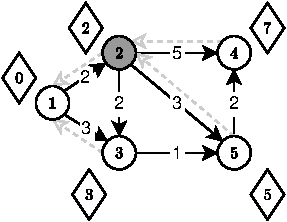
\includegraphics[width=\textwidth]{Chapter_II/TOPOLOGIC-SHORTEST-PATH-Example/b.pdf}
		\caption{}
	\end{subfigure}
	\begin{subfigure}[b]{0.18\textwidth}
		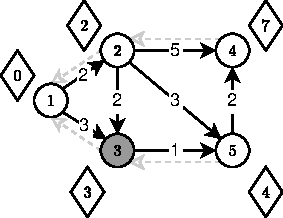
\includegraphics[width=\textwidth]{Chapter_II/TOPOLOGIC-SHORTEST-PATH-Example/c.pdf}
		\caption{}
	\end{subfigure}
	\begin{subfigure}[b]{0.18\textwidth}
		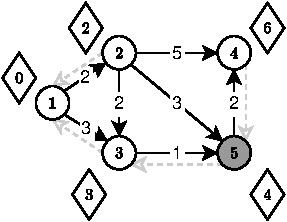
\includegraphics[width=\textwidth]{Chapter_II/TOPOLOGIC-SHORTEST-PATH-Example/d.pdf}
		\caption{}
	\end{subfigure}
	\begin{subfigure}[b]{0.18\textwidth}
		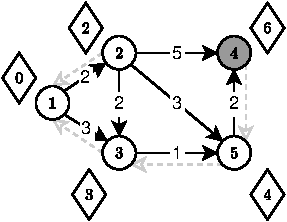
\includegraphics[width=\textwidth]{Chapter_II/TOPOLOGIC-SHORTEST-PATH-Example/e.pdf}
		\caption{}
	\end{subfigure}
	\caption{\textbf{Przykład dla ustalonego porządku topologicznego węzłów: $v_{1}, v_{2}, v_{3}, v_{5}, v_{4}$.}} \label{fig:exampleTopologicalShotrestPath}
\end{figure}

\newpage
\section{Generyczny algorytm Dijkstry}
\label{sec:dijkstraGenericAlgorithm}

Pokazaliśmy w~poprzednich rozdziałach, że kolejność przetwarzania węzłów może mieć ogromny wpływ na szybkość działania algorytmu~--- od przeglądania wierzchołków w~kolejności narzuconej nam przez ich uporządkowanie w~strukturach grafu (w czasie $ O \left( \left| V \right| \cdot \left| E \right| \right)$), aż do badania wierzchołków w~porządku topologicznym ($ O \left( \left| V \right| + \left| E \right| \right)$). Oba te algorytmy miały zasadnicze wady: albo działały w~czasie dużo poniżej naszych oczekiwań, wykonując zatrważającą liczbę niepotrzebnych operacji, albo nie nadawały się do użytku w~sieciach, które my chcemy badać (z nieujemnymi cyklami). W~tym rozdziale przedstawimy kolejny sposób przeglądania wierzchołków grafu $G = \left( V, E \right)$, pokażemy generyczny algorytm na nim opartym, a~także udowodnimy jego poprawność. Bazując na kontrprzykładzie, wykażemy także, że nie działa on dla grafów, które zawierają krawędzie o~ujemnych wagach (a co za tym idzie~--- dla grafów z~ujemnymi cyklami). Algorytm, opracowany przez holenderskiego informatyka Edsgera Dijkstrę~\cite[$4.5$]{Ahuja:1993:NFT:137406}, okaże się podstawą do powstania szeregu jego modyfikacji, którym niejednokrotnie zawdzięcza asymptotycznie szybsze czasy działania, a~które omówimy w~tym rozdziale, skupiając się na ich własnościach.

\subsection{Algorytm Dijkstry}
\label{sub:dijkstraAlgorithm}

Sama idea algorytmu jest bardzo podobna do poprzedniej tj. zakłada wykonywanie relaksacji dla wszystkich krawędzi aktualnie badanych wierzchołków, których to kolejność jest w~specyficzny sposób ustalana. W~przypadku algorytmu Dijkstry mamy regułę, która mówi, że wierzchołki są skanowane w~niemalejącej kolejności ich etykiet (atrybutów $d$~--- odległości węzła od źródła $s$), co wiąże się z~wykorzystaniem w~naszym algorytmie \textbf{kolejek priorytetowych}, które zapewniają nam właśnie taki porządek. Jak się później okaże~--- omawiane modyfikacje algorytmu Dijkstry różnią się głównie jej implementacją~\cite[$2.1$]{OR}.

Przyjmiemy, że mamy dwa zbiory rozłączne: $S$, który na początku działania algorytmu jest pusty (zob. pseudokod \ref{alg:GenericDijksta})~--- do niego trafiać będą przetworzone już wierzchołki~--- oraz $\overline{S}$, w~którym na początku przechowywane są wszystkie węzły. Jak już wspomnieliśmy, algorytm ma za zadanie sekwencyjne pobierać ze zbioru $\overline{S}$ takie wierzchołki $v_{i}$, by $v_{i}.d = \min \left\{ v_{j}.d : v_{j} \in \overline{S} \right\}$, przenosić je do zbioru wierzchołków $S$ oraz wykonywać relaksacje dla każdej krawędzi, która wychodzi z~tego wierzchołka. Oczywiście~--- tak jak w~każdym poprzednim algorytmie~--- na początku inicjalizujemy graf metodą \textsc{INIT-GRAPH} $\left( G, s \right)$. Pseudokod generycznego algorytmu Dijkstry wygląda tak, jak przedstawiono poniżej.

\begin{pseudokod}[!htbp]
\DontPrintSemicolon
\Begin{
	$S \longleftarrow \emptyset $ \;
	$\overline{S} \longleftarrow \left\{ v : v \in V \right\} $ \;
	\While{$\overline{S}$ nie jest pusty} {
		$v \longleftarrow  v_{i} : v_{i}.d = \min \left\{ v_{j}.d : v_{j} \in \overline{S} \right\}$ \;
		$S \longleftarrow S \cup \left\{ v \right\}$ \;
		$\overline{S} \longleftarrow \overline{S} - \left\{ v \right\}$ \;
		\ForEach{$e_{ij} : v_{i} \overset{1} \leadsto v_{j}$}{
			$RELAX \left( v_{i}, v_{j} \right)$ \;
		}
	}
}
\caption{ GENERIC-DIJKSTRA $\left( G, s \right)$\label{alg:GenericDijksta}}
\end{pseudokod}

W faktycznej implementacji linijki $5$--$7$ zwykle zastępuje się operacją $\textrm{\textsc{EXTRACT-MIN}} \left( Q \right)$, gdzie $Q$ to nasza kolejka priorytetowa. Zbioru $S$ zaś w~ogóle się nie uwzględnia, gdyż służy on tylko do celów przeprowadzenia dowodów poprawności tego algorytmu i~wykazania, że jest on poprawnie skonstruowany (niezmiennikiem pętli $4$--$9$ w~tym przypadku będzie $Q = V - S$). Odnajdywaniem najmniejszego elementu (w sensie dystansu wierzchołka do źródła) i~usuwaniem go ze zbioru $\overline{S}$ zajmuje się, wymieniona wyżej, operacja (wtedy $\overline{S} = Q$). Na rysunku \ref{fig:exapleDijkstraDLList} jako kolejkę priorytetową wykorzystano podwójnie wiązaną listę (która oczywiście nie jest najfortunniejszym wyborem), której czas potrzebny na wyciągnięcie z~niej najmniejszego elementu, jest zależny od liczby tych elementów na liście (w najgorszym przypadku $ \left| V \right| $).

\begin{figure}[!h]
	\centering
	\begin{subfigure}[b]{0.3\textwidth}
		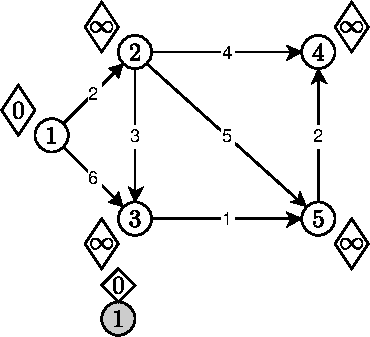
\includegraphics[width=\textwidth]{Chapter_II/DIJKSTRA-DLList/a.pdf}
		\caption{}
	\end{subfigure}%
	\begin{subfigure}[b]{0.3\textwidth}
		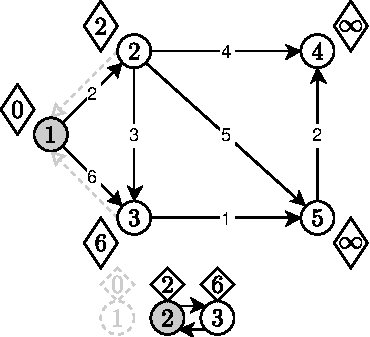
\includegraphics[width=\textwidth]{Chapter_II/DIJKSTRA-DLList/b.pdf}
		\caption{}
	\end{subfigure}
	\begin{subfigure}[b]{0.3\textwidth}
		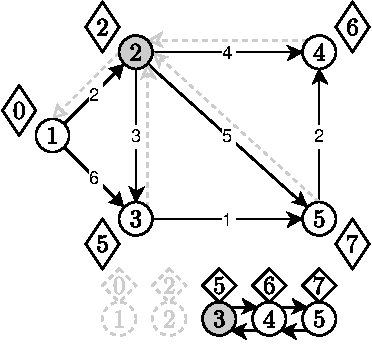
\includegraphics[width=\textwidth]{Chapter_II/DIJKSTRA-DLList/c.pdf}
		\caption{}
	\end{subfigure}
	\begin{subfigure}[b]{0.3\textwidth}
		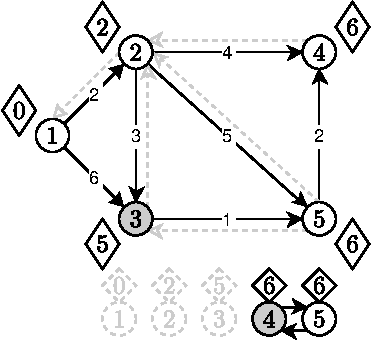
\includegraphics[width=\textwidth]{Chapter_II/DIJKSTRA-DLList/d.pdf}
		\caption{}
	\end{subfigure}%
	\begin{subfigure}[b]{0.3\textwidth}
		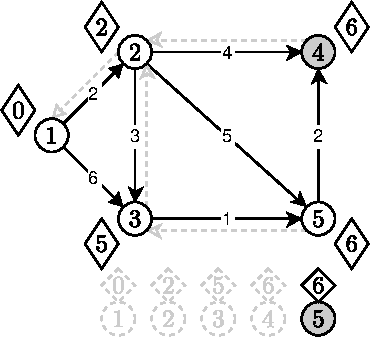
\includegraphics[width=\textwidth]{Chapter_II/DIJKSTRA-DLList/e.pdf}
		\caption{}
	\end{subfigure}
	\begin{subfigure}[b]{0.3\textwidth}
		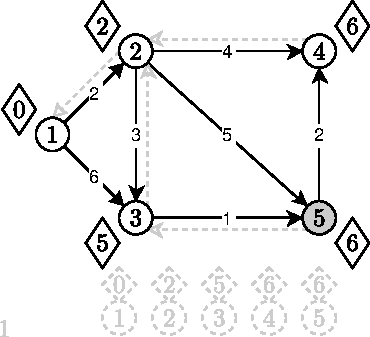
\includegraphics[width=\textwidth]{Chapter_II/DIJKSTRA-DLList/f.pdf}
		\caption{}
	\end{subfigure}
	\caption{\textbf{Działanie algorytmu Dijkstry} \textbf{(a)} Sytuacja po zainicjowaniu grafu $G = \left( V, E \right)$ przez \textsf{INIT-GRAH} ze źródłem $v_{s}.id = 1$. \textbf{(b)} Z~listy dwukierunkowej został wyciągnięty najmniejszy element i~została wykonana operacja \textsc{RELAX} dla krawędzi: $e_{12}$ i~$e_{13}$. Odpowiednio węzły $v_{2}$ i~$v_{3}$ zostały wstawione do kolejki. \textbf{(c)} Najmniejszym elementem na liście był węzeł $v_{2}$. Został usunięty z~kolejki, algorytm wykonał relaksację krawędzi $e_{23}$, $e_{24}$ i~$e_{25}$. Etykieta węzła $v_{3}$ uległa zmniejszeniu. \textbf{(d--f)} Kroki analogiczne jak poprzednie.} \label{fig:exapleDijkstraDLList}
\end{figure}

\subsection{Złożoność obliczeniowa}

Analizując złożoność czasową algorytmu, widzimy że jego główna pętla $4$--$9$ wykonuje się dokładnie $ \left| V \right| $ razy, za każdym razem usuwając z~kolejki priorytetowej dokładnie jeden węzeł, gdzie skanowane węzły nie powtarzają się \footnote{Liczba wykonywanych pętli możemy ograniczyć, kończąc algorytm, gdy z~kolejki zostanie wyjęty taki węzeł $v$, że $v.d = \infty$. Jak wiemy, relaksacja żadnej krawędzi wychodzącej z~takiego węzła nie zmieni nam sytuacji w~grafie, a~z własności kolejki priorytetowej wiemy, że pozostałe elementy $u$ , które w~niej zostały, spełniają $u.d \geqslant v.d = \infty$.}. Następnie, wewnątrz pętli, wyszukiwany jest najmniejszy element w~kolejce~--- czas tej operacji jest naturalnie zależny od wybranego przez nas sposobu jej implementacji i~--- na pożytek naszych rozważań~--- niech zajmuje czas $O \left( \textrm{\textsc{EXTRACT-MIN}} \left( Q \right) \right)$. Takich operacji podczas działania algorytmu wykonamy $ \left| V \right| $. Dla każdego węzła, wyjętego z~kolejki, dla wszystkich łuków, wychodzących z~danych węzłów, wykonywana jest operacja relaksacji~--- łatwo zauważyć, że podczas całej procedury metoda \textsc{RELAX} zostanie wywołana dokładnie $ \left| E \right|$ razy, podczas której może być wymagane zmniejszenie atrybutu $d$ któregoś z~węzłów~--- koszt takiej operacji jest znowu zależny od implementacji kolejki priorytetowej (wraz ze zmniejszeniem się klucza może zajść konieczność przemieszczenia węzła bliżej głowy kolejki) i~dla naszej analizy niech wyniesie $O \left( \textrm{\textsc{DECREASE-KEY}} \left( Q, v, k \right) \right)$, gdzie $k$ to nowy klucz (nowa odległość od źródła $s$~--- $v.d$) węzła $v$. Pozostaje nam jeszcze metoda $\textrm{\textsc{INSERT}} \left( Q, v \right)$, która wstawia nam elementy do kolejki. Czas jej działania jest również zależny od wybranej implementacji kolejki $Q$, zaś miejsce jej wywołania zależne jest już od woli programisty; może on przed rozpoczęciem algorytmu wstawić wszystkie wierzchołki grafu do kolejki (wiersz $3$), bądź też wstawiać je na bieżąco w~chwili, gdy algorytm potrafi już do nich dojść (wtedy podczas relaksacji podejmowana jest decyzja czy wstawić nowy element do kolejki, czy taki już w~kolejce istnieje i~należy tylko zmniejszyć jego klucz oraz~zadbać o~zachowanie prawidłowego porządku w~strukturze danych). Bez względu na preferowane rozwiązanie liczba takich operacji wyniesie dokładnie $ \left| V \right|$, jako że każdy wierzchołek wstawimy do kolejki (i wyjmiemy go z~niej) tylko raz. Reasumując~--- złożoność algorytmu Dijkstry w~uogólnionym przypadku jest ograniczona z~góry przez:

\begin{equation}
O \left( \left| E \right| \cdot O \left( \textrm{\textsc{DECREASE-KEY}} \left( Q, v, k \right) \right) + \left| V \right| \cdot \left[ O \left( \textrm{\textsc{INSERT}} \left( Q, v \right) \right) + O \left( \textrm{\textsc{EXTRACT-MIN}} \left( Q \right) \right) \right] \right)
\end{equation}\label{eq:dijkstraComplexity}.

\textbf{Wąskim gardłem} algorytmu nazywamy taki jego element składowy, który przesądza o~złożoności obliczeniowej całego algorytmu, niejednokrotnie go zwalniając. W~tym przypadku nie ma wątpliwości, że takim elementem w~algorytmie Dijkstry jest zastosowana struktura, odpowiedzialna za wykonywanie tych trzech operacji.

\subsection{Ujemne koszty krawędzi}

Nim udowodnimy poprawność algorytmu Dijkstry, opierając się w znacznej mierze na \cite[$24.6$]{Cormen}, przeanalizujemy jeszcze prosty przykład, w~którym dopuścimy wystąpienie krawędzi o~ujemnym koszcie i~pokażemy, że dla takiego grafu nasz algorytm zwróci błędny wynik.

\begin{figure}[!htbp]
	\centering
	\begin{subfigure}[b]{0.3\textwidth}
		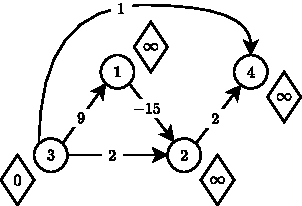
\includegraphics[width=\textwidth]{Chapter_II/DIJKSTRA-NegativeArc/a.pdf}
		\caption{}
	\end{subfigure}%
	\begin{subfigure}[b]{0.3\textwidth}
		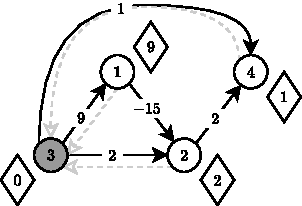
\includegraphics[width=\textwidth]{Chapter_II/DIJKSTRA-NegativeArc/b.pdf}
		\caption{}
	\end{subfigure}
	\begin{subfigure}[b]{0.3\textwidth}
		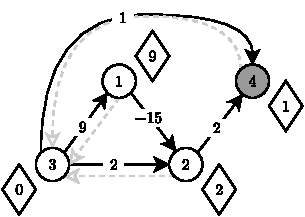
\includegraphics[width=\textwidth]{Chapter_II/DIJKSTRA-NegativeArc/c.pdf}
		\caption{}
	\end{subfigure}
	\begin{subfigure}[b]{0.3\textwidth}
		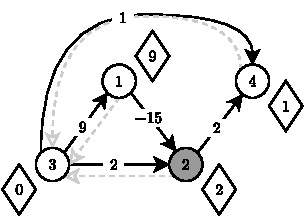
\includegraphics[width=\textwidth]{Chapter_II/DIJKSTRA-NegativeArc/d.pdf}
		\caption{}
	\end{subfigure}%
	\begin{subfigure}[b]{0.3\textwidth}
		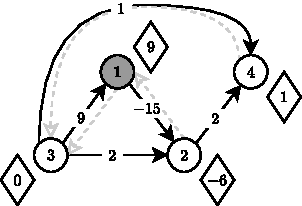
\includegraphics[width=\textwidth]{Chapter_II/DIJKSTRA-NegativeArc/e.pdf}
		\caption{}
	\end{subfigure}
	\caption{\textbf{Działanie algorytmu Dijkstry w~grafie z~ujemnymi kosztami krawędzi}} \label{fig:exapleDijkstraNegativArc}
\end{figure}

Jak powiedzieliśmy, algorytm Dijkstry analizuje wierzchołki grafu $G = \left( V, E \right)$ w~ściśle określonym porządku tj. bada zawsze taki węzeł $v$ , którego $v.d$ jest najmniejsze spośród wszystkich pozostałych, jeszcze nie przeanalizowanych węzłów. Na kolejnych rysunkach zaznaczono kolejność przeglądania węzłów jaka wynika z~tej własności (za węzeł startowy przyjęliśmy $v_{3}$). Widzimy, że algorytm zwrócił błędną ścieżkę dla pary węzłów: $v_{3}$ i~$v_{4}$ (poprawną, najkrótszą ścieżką $v_{3} \overset{*}\leadsto v_{4}$ jest ścieżka $ P = \left \langle v_{3}, v_{1}, v_{2}, v_{4} \right \rangle $ o koszcie $-4$, nie zaś ścieżka $ P^{'} = \left \langle v_{3}, v_{4} \right \rangle $ ) ze względu na wystąpienie w~grafie krawędzi o~ujemnym koszcie. Problemem tutaj jest oczywiście niepoprawna kolejność, w jakiej algorytm otrzymywał informację o wierzchołkach (koszt dotarcia do węzła $v_{2}$ okazuje się w rzeczywistości dużo mniejszy dopiero, gdy algorytm wykona relaksacje dla krawędzi wychodzących z wierzchołka $v_{1}$, który ma najniższy priorytet).
\newpage

\subsection{Poporawność działania}

\begin{figure}[!htbp]
	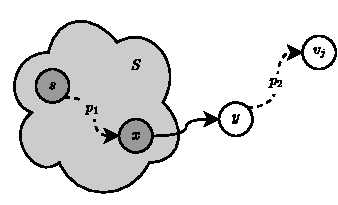
\includegraphics[width=0.3\textwidth]{Chapter_II/ProofOfDijkstra/a.pdf}
	\caption{\textbf{Dowód poprawności algorytmu Dijkstry}} Tuż przed wstawieniem wierzchołka $v_{j}$ do $S$ ten ostatni nie jest pusty. Przerywanymi strzałkami zaznaczono ścieżki $p_{1}$ oraz $p_{2}$, które mogą mieć dowolnie dużą liczbę składowych (w skrajnym przypadku $s = x$ i/lub $y = v_{j}$). Dodatkowo $x \neq y$. Podobny rysunek znajduje się w \cite[$674$]{Cormen}. \label{fig:proofOfDijkstra}
\end{figure}

\begin{proof}
\label{pr:dijkstra}
Załóżmy indukcyjnie, że dla każdego węzła $v_{i}$ w~momencie dodawania go do zbioru wierzchołków przetworzonych $S$ zachodzi $v_{i}.d = \delta \left( s, v_{i} \right)$. Pierwszy krok indukcyjny jest oczywisty, gdyż na samym początku zbiór $S$ jest pusty i~założenie jest prawdziwe. Pierwszym wierzchołkiem, który jest dodawany do tego zbioru, jest wierzchołek $s$ będący źródłem, którego w~oczywisty sposób $s.d = 0 = \delta \left( s, s \right)$ (w grafie dla algorytmu Dijkstry założyliśmy brak krawędzi o~ujemnych długościach). Przyjmijmy nie w~prost, że istnieje w~grafie taki wierzchołek $v_{j}$, dla którego $v_{j}.d \neq \delta \left( s, v_{j} \right)$ w~trakcie jego dodawania do zbioru $S$ i~będzie on pierwszym takim wierzchołkiem, jaki będziemy chcieli do tego zbioru dodać. Wiemy, że $v_{j} \neq s$ oraz, że do takiego wierzchołka na pewno istnieje najkrótsza ścieżka ze źródła $s$ (gdyby tak nie było to odpowiednio wtedy $v_{j}.d = s.d = 0 = \delta \left( s, s \right) = \delta \left( s, v_{j} \right)$ lub $v_{j}.d = \delta \left( s, v_{j} \right) = \infty $~--- z~własności braku ścieżki). Bezpośrednio z~poprzednich spostrzeżeń wynika, że w~momencie dodawania wierzchołka $v_{j}$ do zbioru $S$ ten jest niepusty i~zawiera co najmniej jeden element~--- źródło. Niech istniejąca ścieżka z~$s$ do $v_{j}$ nazywa się $P$. Rozważmy sytuację taką, jaką widać na rysunku \ref{fig:proofOfDijkstra}. Rozbiliśmy na nim ścieżkę $P$ na dwie składowe: $p_{1}$ i~$p_{2}$, gdzie $v_{s} \overset{p_{1}}\leadsto x \overset{1}\leadsto y \overset{p_{2}}\leadsto v_{j}$ oraz pierwsza z~nich składa się tylko z~węzłów należących do zbioru $S$, zaś druga~--- tylko z~węzłów poz tym zbiorem. Dodatkowo, węzeł $y$ jest pierwszym na ścieżce $P$, który jest poza tym zbiorem. Pokażemy teraz, że w~momencie dodawania wierzchołka $v_{j}$ ($v_{j}.d \neq \delta \left( s, v_{j} \right)$) do zbioru $S$ zachodzi $y.d = \delta \left( s, y \right)$. Aby udowodnić ten fakt, wystarczy zauważyć, że skoro wierzchołek $v_{j}$ był pierwszym takim, dla którego zachodzi $v_{j}.d \neq \delta \left( s, v_{j} \right)$, to wstawiając do zbioru $S$ wierzchołek $x$ na pewno $v_x.d = \delta \left( s, x \right)$, a~ze zbieżności (lemat \ref{lem:convergenceProperty}) mamy, że zachodzi również $y.d = \delta \left( s, y \right)$ (w trakcie dodawania wierzchołka $x$ do zbioru $S$ zajdzie relaksacja krawędzi $x \overset{1}\leadsto y$, gdzie wcześniej $v_x.d = \delta \left( s, x \right)$).

Ponieważ na naszym rysunku wierzchołek $y$ występuje na ścieżce $P$ wcześniej od wierzchołka $v_{j}$ i~każda krawędź w~grafie ma koszt nieujemny, to $ \delta \left( s, y \right) \leqslant \delta \left( s, v_{j} \right) $. Z tego wnioskujemy, że:

\begin{equation}
\begin{aligned}
y.d &= \delta \left( s, y \right) \\
&\leqslant \delta \left( s, v_{j} \right) \\
&\leqslant v_{j}.d \; \; \textrm{(z lematu \ref{lem:costUpperBound} o~górnym ograniczeniu)}
\end{aligned}
\end{equation}

Wiemy jednak, że z~własności algorytmu Dijkstry zawsze wybieramy wierzchołek spoza zbioru $S$ o~jak najmniejszej wartości atrybutu $d$~--- skoro oba wierzchołki ($y$ i~$v_{j}$) nie należą do zbioru $S$ w~chwili wyboru wierzchołka $v_{j}$, mamy zagwarantowane, że $v_{j}.d = \min \left\{ v.d : v \notin S \right\}$ (w~szczególności $v_{j}.d \leqslant y.d$). Dodając to ostatnie równanie do szeregu poprzednich nierówności otrzymujemy:

\begin{equation}
y.d = \delta \left( s, y \right) = \delta \left( s, v_{j} \right) = v_{j}.d
\end{equation}

Widzimy, że $ v_{j}.d = \delta \left( s, v_{j} \right) $, co jest sprzeczne z~naszym założeniem (dodanie do zbioru $S$ pierwszego wierzchołka $v_{j}$ o~własności  $v_{j}.d = \delta \left( s, v_{j} \right) $). Rozumowanie jest identyczne w~przypadku, gdyby na ścieżkach $p_{1}$ i/lub $p_{2}$ znajdowała się dowolna liczba węzłów, spełniających nasze założenia. Pokazaliśmy zatem, że dla każdego wierzchołka $v \in V$, w~momencie jego dodawania do zbioru $S$, zachodzi $v.d = \delta \left( s, v \right)$. Algorytm kończy działanie, gdy w~kolejce $Q$ nie ma już żadnych wierzchołków (wszystkie zostały dodane do zbioru $S$), tak więc w~momencie, gdy każdy wierzchołek spełnia $v.d = \delta \left( s, v \right)$, co kończy dowód.
\end{proof}

\section{Podstawowe struktury danych}

Jak pokazaliśmy wcześniej~--- efektywność algorytmu Dijkstry w~głównej mierze zależy od efektywności implementacji struktury, od której będziemy wymagać wykonywania trzech, podstawowych operacji: $\textrm{\textsc{INSERT}} \left( Q, v \right)$, $\textrm{\textsc{EXTRACT-MIN}} \left( Q \right)$ i~$\textrm{\textsc{DECREASE-KEY}} \left( Q, v, k \right)$. Wyspecjalizowanymi strukturami do ich wykonywania są kolejki priorytetowe, choć~--- jak mogliśmy się już przekonać~--- inne struktury, takie jak tablice, listy jednokierunkowe czy podwójnie wiązane (ang. \textit{double-linked lists}), także umożliwiają nam poprawną konstrukcję algorytmu Dijkstry. Korzystając z~nich, musimy jednak płacić cenę za ich wysoką nieefektywność (dla listy dwukierunkowej, wykorzystanej przy omawianiu algorytmu, wyszukanie najmniejszego elementu kosztuje nas proporcjonalnie do liczby wierzchołków, znajdujących się na niej w~trakcie wyszukiwania). Jeżeli spojrzymy na złożoność algorytmu Dijkstry (\ref{eq:dijkstraComplexity}), natychmiastowo uzyskamy górne ograniczenie na poziomie $ O \left( \left| V \right| ^{2} \right)$, co niewiele oddala nas złożoności tak prostego algorytmu, jakim jest algorytm Bellmana-Fora.


Mówiąc o~różnych wcieleniach algorytmu Dijkstry, nie sposób jest więc nie poruszyć tematu podstawowych struktur danych, jakie możemy wykorzystać do implementacji różnych kolejek priorytetowych, ich właściwości i~czasu działania podstawowych operacji, których wykonywanie dane struktury umożliwiają~--- w~szczególności $\textrm{\textsc{INSERT}} \left( Q, v \right)$, $\textrm{\textsc{EXTRACT-MIN}} \left( Q \right)$ i~$\textrm{\textsc{DECREASE-KEY}} \left( Q, v, k \right)$. W~niniejszym rozdziale omówimy takie struktury jak: kopce binarne (w uogólnionym spojrzeniu na kopce $R$-arne), kopce Fibonacciego, kolejki z~przepełnieniem oraz szereg innych pomysłów, opartych o~kontenery, zwane dalej kubełkami (ang. \textit{buckets}~\cite[$4.6$,$4.8$]{Ahuja:1993:NFT:137406}).

\section{Struktury oparte na kopcach}

Jedną ze struktur, przystosowanych do operacji charakterystycznych dla kolejki priorytetowej, jest kopiec (ang. \textit{heap}). Jego najogólniejszą własnością jest to, że operacja, zwracająca najmniejszy (lub największy) element, który znajduje się w~kopcu, działa w~czasie stałym i~polega na odwołaniu się do szczytu takiego kopca. Kopce to szczególne przypadki drzew, gdzie pomiędzy rodzicem a~potomkami zwykle jest ustalona stała relacja (w przypadku, który nas interesuje, klucze przechowywane przez potomków węzła $v$ powinny być zawsze większe od klucza rodzica: $v.d \leqslant v_{i} : v_{i}.\Pi = v$~--- właściwość kopca typu \textsc{min}). Przedstawimy dwa, powszechnie znane rodzaje kopców: zwykły, do którego implementacji wykorzystamy tablicę, rozszerzając powszechną implementację jego binarnej wersji, oraz kopiec Fibonacciego, który~--- jak się okaże~--- pomimo swojej teoretycznej przewagi w~szybkości wykonywania poszczególnych operacji, w~praktyce często działa wolniej od wspomnianej wcześniej wersji, znacznie prostszej w implementacji.

\subsection{Kopiec R-arny}

Kopien $R$-arny jest uogólnieniem kopca binarnego~--- podczas gdy dla tego drugiego każdy rodzic może posiadać do $2$ potomków, w~pierwszym przypadku takich węzłów rodzic może mieć od $0$ do $R$, co zauważalnie zmniejsza wysokość takiego kopca (kosztem jego szerokości). Poniższa tabelka przedstawia koszty poszczególnych operacji dla kopca binarnego i~$R$-arnego:

\begin{center}
	\begin{tabular}{ccc}
		& \multicolumn{2}{c}{Kopiec} \\
		\cline{2-3}
		Operacja & binarny & $R$-arny \\
		\hline
		$\textrm{\textsc{INSERT}} \left( Q, v \right)$ & $O \left( \log \left( n \right) \right)$ & $O \left( \log_{R} \left( n \right) \right)$ \\
		$\textrm{\textsc{EXTRACT-MIN}} \left( Q \right)$ & $O \left( \log \left( n \right) \right)$ & $O \left( R \cdot \log_{R} \left( n \right) \right)$ \\
		$\textrm{\textsc{DECREASE-KEY}} \left( Q, v, k \right)$ & $O \left( \log \left( n \right) \right)$ & $O \left( \log_{R} \left( n \right) \right)$  \\
		\hline
	\end{tabular}
\end{center}

\subsubsection{Implementacja}

Algorytm wyszukiwania najkrótszych ścieżek oparty na strukturze $D$-arnego kopca jest jedynym algorytmem, który nie wymaga od nas tworzenia dodatkowych struktur. Jak dobrze wiemy, jedną z~właściwości kopców jest ich zdolność do pracy w~miejscu tj. nie wykorzystywania dodatkowej pamięci podczas działania. Pod pojęciem naszego grafu $G = \left( V, E \right)$ kryje się tablica $tab \left[ 1 \cdots \left| V\right| \right]$, przechowująca wierzchołki indeksowane ich identyfikatorami ($tab[i]=v_{i}$), oraz listy sąsiedztwa, które są przyporządkowane do każdego z~takich węzłów. Aby skorzystać z~właściwości kopca, będziemy chcieli zbudować jego strukturę bezpośrednio na wspomnianej tablicy węzłów tj. kopiec o~$k$ elementach będziemy chcieli przedstawić jako tablica $vertices \left[ 1 \cdots k \right]$. W~takiej sytuacji, jeżeli dowolny wierzchołek $v$ znajduje się na pozycji $i <= k $ w~tablicy $tab$, to znaczy, że w~którymś momencie został on wstawiony do naszej kolejki priorytetowej i~nie opuści jej, dopóki nie stanie się on najmniejszy spośród tych $k$ elementów. Aby jednak nie stracić informacji o~pierwotnym rozmieszczeniu wierzchołków w~tablicy $tab$, będziemy chcieli wprowadzić pomocniczą tablicę $heapIDArray \left[ 1 \cdots \left| V\right| \right]$, której to wartości będą odzwierciedlać faktyczne rozmieszczenie wierzchołków w~$tab$ po modyfikacjach ($tab \left[ heapIDArray \left[ i \right] \right] = v_{i}$), jakich dopuści się na niej nasza kolejka priorytetowa (indeksami tablicy $tab$ pierwotnie były identyfikatory wierzchołków, a~ich nie możemy zmieniać).

Zasada działania takiego kopca nie różni się niczym od zastosowania takiej samej struktury do posortowania $n$ liczb, gdzie rozmiar kopca monotonicznie rośnie w~trakcie jego budowania a~następnie maleje w~czasie działania takiego algorytmu. W~naszym przypadku liczba jego elementów może się zwiększać jak i~zmniejszać w~dowolnej kolejności~--- jeżeli się zwiększa, to ostatni element w~części tablicy należącej do powiększonego kopca zamieniamy z~elementem, który chcemy faktycznie do niego wstawić, następnie ,,wypychając'' go ku górze (analogiczna procedura jest wykonywana podczas powiększania kopca w~czasie jego budowania dla algorytmu sortowania). W przypadku odwrotnym (jeżeli rozmiar kopca maleje)~--- zachowanie, w~porównaniu z~algorytmem sortującym, jest identyczne.

\begin{figure}[!htbp]
	\centering
	\begin{subfigure}[b]{0.33\textwidth}
		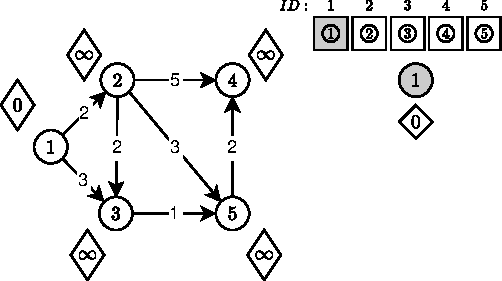
\includegraphics[width=\textwidth]{Chapter_II/R-HEAP-Example/a.pdf}
		\caption{}
	\end{subfigure}%
	\begin{subfigure}[b]{0.33\textwidth}
		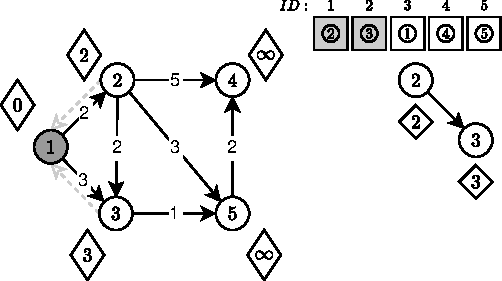
\includegraphics[width=\textwidth]{Chapter_II/R-HEAP-Example/b.pdf}
		\caption{}
	\end{subfigure}
	\begin{subfigure}[b]{0.33\textwidth}
		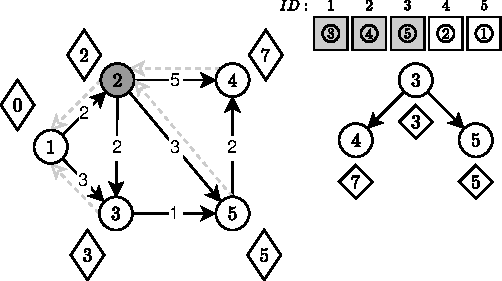
\includegraphics[width=\textwidth]{Chapter_II/R-HEAP-Example/c.pdf}
		\caption{}
	\end{subfigure}
	\begin{subfigure}[b]{0.33\textwidth}
		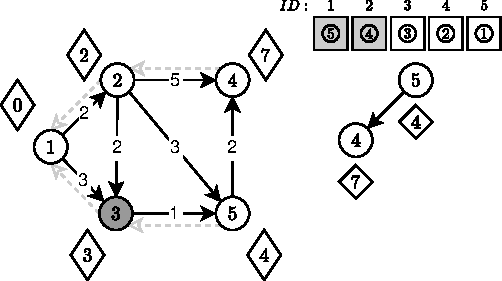
\includegraphics[width=\textwidth]{Chapter_II/R-HEAP-Example/d.pdf}
		\caption{}
	\end{subfigure}%
	\begin{subfigure}[b]{0.33\textwidth}
		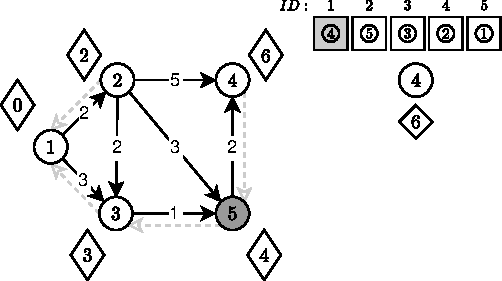
\includegraphics[width=\textwidth]{Chapter_II/R-HEAP-Example/e.pdf}
		\caption{}
	\end{subfigure}
	\begin{subfigure}[b]{0.33\textwidth}
		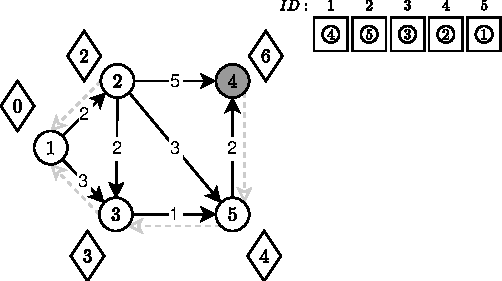
\includegraphics[width=\textwidth]{Chapter_II/R-HEAP-Example/f.pdf}
		\caption{}
	\end{subfigure}
	\caption{\textbf{Działanie algorytmu Dijkstry w~oparciu o~kopiec $R$-arny} \textbf{(a)} Sytuacja po zainicjowaniu grafu $G$ przez \textsf{INIT-GRAH} ze źródłem $v_{1}$. W~tablicy na szaro zaznaczone są elementy należące do kopca, przedstawionego poniżej. Niech $k$ oznacza rozmiar kopca, tablica $tab$ jest indeksowana od $1$. \textbf{(b)} Z~kopca zostaje usunięty węzeł $v_{1}$ ($k=0$). W~wyniku relaksacji na kopiec zostaje przeniesiony węzeł $v_{2}$ ($k=1$ i~$tab \left[ k \right] = v_{2}$), zaś na stare miejsce wstawionego węzła zostaje przeniesiony węzeł $v_{1}$. Analogicznie na koniec kopca wstawiany jest $v_{3}$  ($k=2$, $tab \left[ k \right] = v_{3}$), w~wyniku czego $tab \left[ 3 \right] = v_{1}$. \textbf{(c)} Z~kopca zostaje pobrany węzeł $v_{2}$ a~na szczyt stosu zostaje przeniesiony ostatni element w~kopcu ($v_{3}$). W~wyniku relaksacji krawędzi wychodzących z~pobranego węzła do kopca zostają dodane węzły: $v_{4}$ i~$v_{5}$. Tablica $tab$ zmienia się odpowiednio: $\left\{ 3 \right\} \left[ 2 \right]  \left[ 1 \right]  \left[ 4 \right]  \left[ 5 \right] \rightarrow \left\{ 3 \right\} \left\{ 4 \right\}  \left[ 1 \right]  \left[ 2 \right]  \left[ 5 \right] \rightarrow \left\{ 3 \right\} \left\{ 4 \right\}  \left\{ 5 \right\}  \left[ 2 \right]  \left[ 1 \right]$, gdzie w~klamrach ,,$\left\{\right\}$''~ zostały zaznaczone węzły znajdujące się w~kopcu. Żadna operacja nie narusza własności kopca. \textbf{(d)} Wybrano kolejny węzeł ze szczytu stosu: $v_{3}$, zamieniono go z~ostatnim elementem w~kopcu i~zmniejszono jego rozmiar ($k=2$). Zachowana jest własność kopca. W~wyniku relaksacji zostają zmienione atrybuty: $v_{5}.\Pi = v_{3}$ i~$v_{5}.d = 4$. \textbf{(e--f)} Z~kopca zostaje zabrany jego najmniejszy element: $v_{5}$ i~wykonywana jest operacja \textsf{RELAX} dla krawędzi z~niego wychodzących. Na szczyt kopca zostaje wstawiony jego ostatni element ($k=1$). Własność kopca jest zachowana.} \label{fig:exampleDHeap}
\end{figure}

\subsubsection{Złożoność obliczeniowa}

Uzupełniając wzór \ref{eq:dijkstraComplexity} na ogólną złożoność generycznego algorytmu Dijkstry z~wykorzystaniem kolejek priorytetowych dla kopców $R$-arnych, natychmiast otrzymujemy $O \left( m \cdot \log_{d} \left( n \right) + n \cdot \left[ \log_{d} \left( n \right) + d \cdot \log_{d} \left( n \right) \right] \right) = O \left( m \cdot \log_{d} \left( n \right) + n \cdot d \cdot \log_{d} \left( n \right) \right) $ (dla przejrzystości zapisu przyjęliśmy $ n = \left| V\right|$ i~$ m = \left| E \right|$). Dla kopca binarnego mamy: $O \left( m \cdot \log \left( n \right) + n \cdot \log \left( n \right) \right) = O \left( m \cdot \log \left( n \right) \right) $ dla $m \geqslant n $ (stałe wyeliminowaliśmy). Przypomnijmy sobie, że naiwna implementacja algorytmu Dijkstry miała złożoność $ O \left( m + n^{2} \right) = O \left( n^{2} \right)$. Łatwo zauważyć, że dla bardzo gęstych grafów (gdzie $ m = \Omega \left( n^{2} \right) $) nasz nowy algorytm asymptotycznie staje się wolniejszy nawet od wspomnianej, naiwnej implementacji, jednak sytuacja zmienia się na korzyść kopców, gdy liczba krawędzi w~grafie jest z~góry ograniczona przez $ O \left( \frac{n^{2}}{ \log \left( n \right) } \right)$ ( wtedy $ O \left( m \cdot \log \left( n \right) \right) \leqslant O \left( \frac{n^{2}}{\log \left( n \right)} \cdot \log \left( n \right) \right) = O \left( n^{2} \right)$).

Z kolei dla kopców, których arność jest większa ($d \geqslant 2$), mamy: $O \left( m \cdot \log_{d} \left( n \right) + n \cdot d \cdot \log_{d} \left( n \right) \right) $. Z~tego bezpośrednio wynika, że optymalną wartością parametru $d$ jest $ \max \left\{ 2, \left \lceil \frac{m}{n} \right \rceil \right\} $, dla którego zrównują nam się obie strony sumy otrzymanej wcześniej złożoności ($ n \cdot \frac{m}{n} \cdot \log_{d} \left( n \right) = m \cdot \log_{d} \left( n \right) $). Otrzymaliśmy złożoność algorytmu Dijkstry, opartego o~kopce $R$-arne, który znów~--- w~zależności od sieci, dla której go zastosujemy, będzie porównywalny albo do podstawowej, naiwnej implementacji tego samego algorytmu ( dla sieci gęstych, gdzie $ m = \Omega \left( n^{2} \right)$ mamy: $O \left( m \cdot \log_{d} \left( n \right) \right) = O \left( n^{2} \cdot \log_{\frac{n^{2}}{n}} \left( n \right) \right) = O \left( n^{2} \cdot \log_{n} \left( n \right) \right) = O \left( n^{2} \right)$), albo do algorytmu opartego na kopcu binarnym (w przypadku, gdy sieć jest bardzo rzadka). Dla tej drugiej możliwości otrzymujemy natychmiastowo złożoność $O \left( n \cdot \log \left( n \right) \right)$ dla $m = O \left( n \right)$~\cite[$2.2$]{OR}.

Co więcej, jeżeli założymy $m = \Omega \left( n^{1+\epsilon} \right)$ dla $\epsilon > 0$ i~$d = \left \lceil \frac{m}{n} \right \rceil > 2$, to będziemy mogli wyprowadzić następujący ciąg równości:

\begin{equation}
	\begin{aligned}
		O \left( m \cdot \log_{d} \left( n \right) \right) &= O \left( m \cdot \frac{\log \left( n \right)}{\log \left( d \right)} \right) \; \; \left( \textrm{zamiana podstawy logarytmu} \right) \\
		&= O \left( m \cdot \frac{\log \left( n \right)}{\log \left( n^{\epsilon} \right)} \right) \; \; \left( d = \left \lceil \frac{m}{n} \right \rceil = \frac{n^{1+\epsilon}}{n} \right) \\
		&= O \left( m \cdot \frac{\log \left( n \right)}{ \epsilon \cdot \log \left( n \right)} \right) \; \; \left( \log_{a} \left( b^{c} \right) = c \cdot \log_{a} \left( b \right) \right) \\
		&= O \left( \frac{m}{\epsilon} \right) \\
		&= O \left( m \right) \; \; \left( \frac{1}{\epsilon} \textrm{jest stałą.} \right)
	\end{aligned}
\end{equation}


Jeśli $\epsilon = 1$, to $ m = \Omega \left( n^{2} \right)$ a~ten wariant analizowaliśmy już wcześniej. Widzimy więc, że w~zależności od gęstości grafu te same algorytmy mogą zachowywać się zupełnie inaczej, a~co za tym idzie~--- nie jesteśmy w~stanie wskazać jednej implementacji algorytmu wyszukiwania najkrótszych ścieżek, która działałaby równie szybko (w porównaniu do reszty algorytmów) dla każdej z~możliwych sieci.

\subsubsection{Drzewa}

Strukturami bardzo podobnymi do kopców są drzewa $K$-arne~\cite[$3.1$]{TaDS}~--- należy wręcz powiedzieć, że kopce są \textbf{pełnymi drzewami} (ang. \textit{complete tree}), podczas gdy struktura zwykłego drzewa jest mniej rygorystyczna. Pełnym drzewem $R$-arnym (jakim jest kopiec tej samej arności) nazywamy takie drzewo, na poziomach którego (poza ostatnim) wszystkie węzły mają dokładnie $R$ potomków. W~przypadku drzew $K$-arnych każdy węzeł może mieć co najwyżej $K$ węzłów potomnych, co nie musi wcale oznaczać, że stworzone tak drzewo, jest drzewem pełnym. Obie struktury (kopce i drzewa) da się zaimplementować przy wykorzystaniu zwykłych tablic, choć oczywiście pomiędzy kolejnymi elementami takiej tablicy mogą pojawić się miejsca puste, gdy któryś z~węzłów drzewa ma mniej niż $K$ potomków. Inne są także założenia samych struktur: każdy węzeł w~drzewie $K$-arnym posiada tyleż potomków w~ściśle zdefiniowanym porządku (niemalejącym lub nierosnącym), zaś reguły, odnoszące się do kopców nic o~takim porządku nie mówią~--- jedyna własność, która musi zostać spełniona dla węzła to przewyższanie jego priorytetem wszystkich swoich potomków (bądź posiadanie najmniejszego priorytetu pośród nich w~przypadku kopca typu \textit{min}). Bezpośrednią konsekwencją tych własności są różne zastosowania wymienionych struktur danych: 

\begin{center}
	\begin{savenotes}
		\begin{tabular}{ccccc}
			& \multicolumn{2}{c}{Drzewo} & \multicolumn{2}{c}{Kopciec} \\
			\cline{2-5}
			Operacja & binarne\footnote{Przedstawiono czasy dla odpowiednio: drzew zbalansowanych (takich jak RBT, AVL) i~drzew niezbalansowanych, dla których pesymistyczna wysokość wynosi $O \left( n\right)$.} & $K$-arne & binarny & $R$-arny \\
			\hline
			$\textrm{\textsc{INSERT}} \left( Q, v \right)$ & $ O \left( \log \left( n \right) \right)$ / $ O \left( 1 \right) $ & $O \left( K \cdot \log_{K} \left( n \right) \right)$ & $O \left( \log \left( n \right) \right)$ & $O \left( \log_{R} \left( n \right) \right)$ \\
			$\textrm{\textsc{EXTRACT-MIN}} \left( Q \right)$ & $ O \left( \log \left( n \right) \right)$  / $ O \left( n \right) $ & $ O \left( \log_{K} \left( n\right) \right)$ & $O \left( \log \left( n \right) \right)$ & $O \left( R \cdot \log_{R} \left( n \right) \right)$ \\
			$\textrm{\textsc{DECREASE-KEY}} \left( Q, v, k \right)$ & $ O \left( \log \left( n \right) \right)$  / $ O \left( 1 \right) $ & $O \left( K \cdot \log_{K} \left( n \right) \right)$ & $O \left( \log \left( n \right) \right)$ & $O \left( \log_{R} \left( n \right) \right)$  \\
			$\textrm{\textsc{SEARCH}} \left( Q, k \right)$ & $ O \left( \log \left( n \right) \right)$ / $ O \left( n \right) $ & $O \left( K \cdot \log_{K} \left( n \right) \right)$ & $O \left( n \right)$ & $ O \left( n \right) $  \\
			\hline
		\end{tabular}
	\end{savenotes}
\end{center}

strukturę drzew stosuje się dla problemów, gdzie nacisk jest kładziony na wyszukiwanie elementów po ich właściwościach, zaś wybieranie minimum jest sprawą drugorzędną. Odwrotna sytuacja występuje w~przypadku kopców, które w~żaden sposób nie wspierają operacji wyszukiwania, sprowadzając ją do przeszukania całej tablicy reprezentującej kopiec. Innymi słowy: drzewa $K$-arne nie są przystosowane do pełnienia roli kolejki priorytetowej. Przywołując wzór na ogólną złożoność algorytmu Dijkstry ( \ref{eq:dijkstraComplexity} ):

\begin{equation}
O \left( m \cdot O \left( \textrm{\textsc{DK}} \left( Q, v, k \right) \right) + n \cdot \left[ O \left( \textrm{\textsc{I}} \left( Q, v \right) \right) + O \left( \textrm{\textsc{EM}} \left( Q \right) \right) \right] \right)\textrm{,}
\end{equation}\label{eq:dijkstraComplexityShort}

i porównując czasy wykonywanych operacji, dojdziemy do następujących złożoności:

\begin{itemize}
\item $ O \left( \left( n + m \right) \cdot \log \left( n \right) \right)$  dla zbalansowanych drzew przeszukiwań binarnych,
\item $ O \left( m + n^{2} \right) = O \left( n^{2} \right) $ dla niezbalansowanych drzew przeszukiwań binarnych,
\item $ O \left( \left( n + m \right) \cdot K \cdot \log_{K} \left( n \right) \right)$  dla zbalansowanych drzew $K$-arnych,
\end{itemize}

gdzie złożoności algorytmu wyszukiwania najkrótszych ścieżek w~oparciu o~kopce policzyliśmy w~poprzednim podrozdziale i~wynosiły one: $ O \left( \left( n + m \right) \cdot \log \left( n \right) \right) $ i~$ O \left( m \cdot \log_{d} \left( n \right) \right) $~--- odpowiednio dla kopców binarnych i~$R$-arnych. Na podstawie powyższego zestawienia możemy podejrzewać, że struktura zbalansowanych drzew binarnych jest w~pewnym stopniu konkurencyjna dla kopców tej samej arności \footnote{Jeżeli byśmy chcieli uzyskać dla zbalansowanych drzew $K$-arnych takie samo oszacowanie na asymptotyczną złożoność obliczeniową, musielibyśmy przyjąć $K = \frac{m}{m+n}$ (wtedy $O \left( \left( n + m \right) \cdot K \cdot \log_{K} \left( n \right) \right) = O \left( m \cdot \log_{K} \left( n \right) \right) $), lecz nie możemy mieć struktury, której współczynnik rozgałęzienia ($d$) jest mniejszy od dwóch (przypadek drzewa binarnego)}, jednak w~tej analizie nie braliśmy w~ogóle pod uwagę stałych czynników, jakie pojawiają się podczas wykonywania wszystkich przeanalizowanych operacji, a~które przemawiają na niekorzyść zbalansowanych drzew przeszukiwań~--- te struktury (takie jak Drzewo Czerwono-Czarne czy Adelsona-Velskiego-Landisa) są znacznie bardziej złożone, przez co wymagają nie tylko więcej pamięci na przechowywanie danych, ale też wykazują się mniejszą efektywnością niż prostsze struktury o~tych samych asymptotycznych czasach działania. Jak się przekonamy w~następnym rozdziale, prawidłowość ta dotyczy również kopców Fibonacciego, które pomimo lepszych wyników teoretycznych, nie sprawdzą się jako kolejka priorytetowa dla algorytmu Dijkstry właśnie ze względu na możliwość zastąpienia tej struktury przez dużo prostsze i~mniej skomplikowane rozwiązania.

\subsection{Kopiec Fibonacciego}

Przedstawiona w~tym rozdziale implementacja algorytmu Dijkstry jako kolejkę priorytetową będzie wykorzystywać jedną z~bardziej złożonych struktur danych, jakie będziemy omawiać~--- kopce Fibonacciego. Zaletą jej wykorzystania okaże się amortyzacyjnie lepszy czas wykonywania dla dwóch podstawowych operacji, wykorzystywanych podczas działania naszego algorytmu~--- $\textrm{\textsc{INSERT}} \left( Q, v \right)$ i~$\textrm{\textsc{DECREASE-KEY}} \left( Q, v, k \right)$.


Dodatkowo, aby jeszcze przyśpieszyć działanie podstawowej wersji implementacji kopca Fibonacciego, możemy dostosować ją do właściwego środowiska, w~którym to oparta na kopcu kolejka priorytetowa będzie wykorzystywana. Pierwszą rzeczą, jaką możemy zauważyć to sposób zmiany liczby elementów, które znajdują się na kopcu~--- w~odróżnieniu od algorytmu wyszukiwania najkrótszych ścieżek dla danego grafu $ G = \left( V, E \right)$, gdzie liczba węzłów jest z~góry znana, dla ogólnego przypadku nie jesteśmy w~stanie nic powiedzieć o~maksymalnej liczbie elementów, jakie znajdą się na kopcu. Konsekwencją tej niewiedzy jest konieczność rezerwowania dodatkowej pamięci dla pomocniczych tablic za każdym razem, gdy wykonujemy operację $\textrm{\textsc{EXTRACT-MIN}} \left( Q \right)$. Choć rozmiar takich tablic jest z~góry znany i~wynosi on $ \left \lfloor \log_{\Phi} \left( n \right) \right \rfloor $ to bez znajomości maksymalnej wartości parametru $n$ nie jesteśmy w~stanie tego faktu w~jakikolwiek sposób wykorzystać~\cite[$19.4$]{Cormen}. Inaczej jest w~przypadku, gdy mamy dany graf $G$, którego liczba wierzchołków wynosi dokładnie $ \left| V \right|$, co przekłada się na maksymalną liczbę elementów, jakie jednocześnie mogą znaleźć się na kopcu Fibonacciego~--- wówczas z~każdą operacją $\textrm{\textsc{EXTRACT-MIN}} \left( Q \right)$ korzystamy z~tej samej tablicy pomocniczej $A \left[ 1 \cdots \left \lfloor \log_{\Phi} \left( n \right) \right \rfloor \right]$, którą ,,czyścimy'' pod sam koniec procedury, budując~--- zgodnie z~podstawowym algorytmem~--- nową listę korzeni kopca Fibonacciego (iterując po całej tablicy i~dodając trzymane w~niej drzewa ukorzenione do głównej listy, zaś elementy samej tablicy~--- zerując)~\cite[$523$--$524$]{Cormen}. Inną, bardziej oczywistą modyfikacją, jest wykorzystanie faktu, iż każda lista, która znajduje się w~wewnętrznej strukturze kopca, jest cykliczną listą dwukierunkową, co znów (w~przypadku wykonywania procedury $\textrm{\textsc{EXTRACT-MIN}} \left( Q \right)$) pozwoli nam zaoszczędzić trochę czasu podczas pierwszych kroków tego algorytmu (zamiast usuwać najmniejszy element $v$ z~listy korzeni i~iteracyjnie przepinać potomków tego węzła do wspomnianej listy, możemy ,,rozerwać'' obie listy w~wybranym przez nas punkcie a~następnie połączyć w~czasie $O \left( 1 \right)$. Usuwanie powiązań między potomkami usuwanego węzła możemy tymczasowo zignorować~--- podstawowa wersja algorytmu podczas przepinania węzłów $u$, takich że $ u.\Pi = v$ ustawia te parametry na wartość \KwNull. Podkreślić należy słowo: ,,tymczasowo''~, gdyż ta czynność zostanie wykonana w~momencie rekonstrukcji kopca Fibonacciego z~drzew, przechowywanych w~tablicy $A \left[ 1 \cdots \left \lfloor \log_{\Phi} \left( n \right) \right \rfloor \right]$~--- wiedząc, że każdy jej element przechowuje wskaźnik do przyszłego węzła na liście korzeni, będziemy dla każdego elementu z~tablicy $A$ dodatkowo niszczyć wskazanie tego węzła na jego rodzica, którego nie zniszczyliśmy wcześniej.).

\begin{figure}[!htbp]
	\centering
	\begin{subfigure}[b]{0.45\textwidth}
		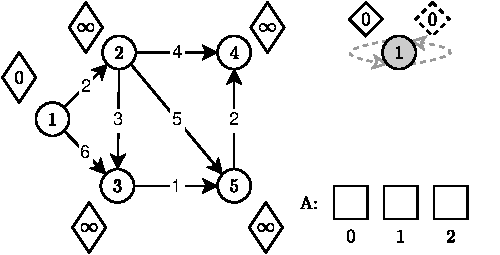
\includegraphics[width=\textwidth]{Chapter_II/FIBONACCI-Example/a.pdf}
		\caption{}
	\end{subfigure}%
	\begin{subfigure}[b]{0.45\textwidth}
		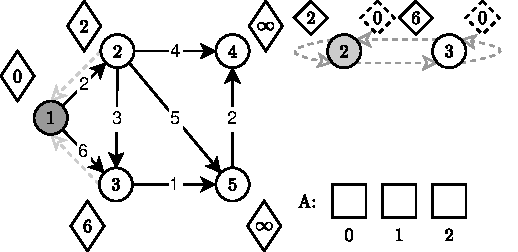
\includegraphics[width=\textwidth]{Chapter_II/FIBONACCI-Example/b.pdf}
		\caption{}
	\end{subfigure}
	\begin{subfigure}[b]{0.45\textwidth}
		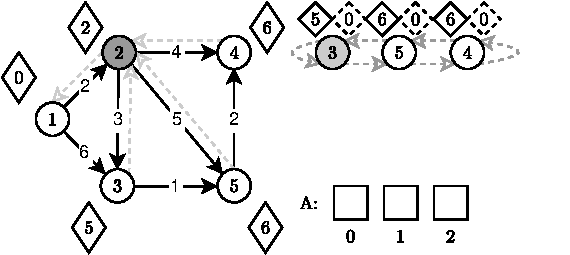
\includegraphics[width=\textwidth]{Chapter_II/FIBONACCI-Example/c.pdf}
		\caption{}
	\end{subfigure}%
	\begin{subfigure}[b]{0.45\textwidth}
		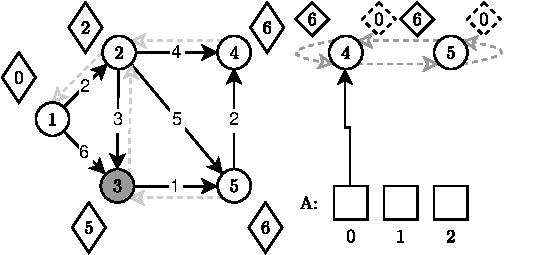
\includegraphics[width=\textwidth]{Chapter_II/FIBONACCI-Example/d.pdf}
		\caption{}
	\end{subfigure}
	\caption{\textbf{Działanie algorytmu Dijkstry w~oparciu o~kopiec Fibonacciego} \textbf{(a)}  Sytuacja po zainicjowaniu grafu $G = \left( V, E \right)$ przez \textsf{INIT-GRAH} ze źródłem $v_{s}.id = 1$. Przerywanymi strzałkami odwzorowane są relacje między węzłami na kopcu Fibonacciego. W~rombach od lewej dla każdego węzła $v$ kolejno przedstawione są jego atrybuty: $v.d$ i~$v.deg$. Szarym kolorem zaznaczono węzeł, który aktualnie jest minimalnym węzłem w~kopcu. \textbf{(b)} Usunięto z~kopca jego najmniejszy węzeł: $v_{1}$. W~wyniku relaksacji do listy korzeni kopca Fibonacciego zostały dodane węzły $v_{2}$~--- ustawiony jako węzeł minimalny w~momencie, gdy był on jedynym elementem na kopcu~--- oraz $v_{3}$. \textbf{(c)} Wykonano relaksację dla następnego, wyjętego z~kopca, węzła $v_{2}$. W~kopcu pozostał tylko jeden wierzchołek $v_{3}$, który stał się tym samym jego najmniejszym elementem. W~wyniku relaksacji do kopca zostały dodane nowe elementy: $v_{5}$ oraz $v_{4}$. \textbf{(d)} Usunięto najmniejszy węzeł z~kopca: $v_{3}$. Po tej operacji na kopcu zostało więcej niż jeden element, więc wykonujemy operację $\textrm{\textsc{CONSOLIDATE}} \left( Q \right)$. Przeglądamy kolejno węzły $v$ na liście korzeni i jeżeli $A \left[ v.deg \right] = \KwNull $ (zaczynamy od węzła $v_{4}$, $v_{4}.deg = 0$), to zapamiętujemy w~$A \left[ v.deg \right]$ korzeń drzewa $v$. Skanujemy kolejny węzeł na liście korzeni: $v_{5}$. } \label{fig:exampleFibonacci1}
\end{figure}
\newpage

\begin{figure}[!htbp]
	\ContinuedFloat
	\centering
	\begin{subfigure}[b]{0.45\textwidth}
		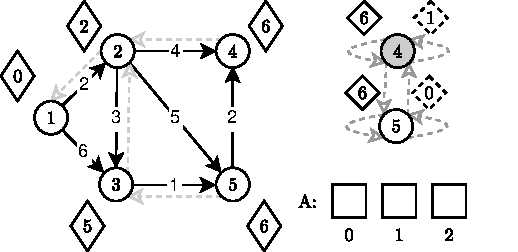
\includegraphics[width=\textwidth]{Chapter_II/FIBONACCI-Example/e.pdf}
		\caption{}
	\end{subfigure}%
	\begin{subfigure}[b]{0.45\textwidth}
		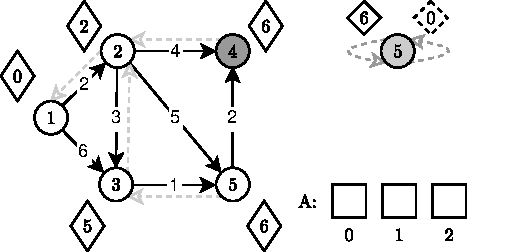
\includegraphics[width=\textwidth]{Chapter_II/FIBONACCI-Example/f.pdf}
		\caption{}
	\end{subfigure}
	\caption{ \textbf{(e)} W~przypadku, gdy dla skanowanego elementu ($v_{5}$) zachodzi warunek przeciwny ($A \left[ v.deg \right] \neq \KwNull $) tworzymy nowe drzewo typu \textit{min}, łącząc to o~korzeniu w~aktualnie badanym wierzchołku z~drzewem, na którego korzeń wskazuje element $A \left[ v.deg \right]$. Korzeniem nowego drzewa zostaje węzeł o~mniejszym kluczu, zaś drzewo, mające korzeń w~drugim węźle, staje się potomkiem tego pierwszego. W~tym przypadku oba korzenie drzew ($v_{4}$ i~$v_{5}$) mają te same priorytety ( $v_{4}.d = v_{5}.d$)~--- korzeniem nowego drzewa staje się wcześniej badany węzeł $v_{4}$ a~jego stopień zostaje zwiększony o~$1$. Korzeń nowo powstałego drzewa jest zapamiętywany w~$A \left[ v_{4}.deg \right]$ (jeśli przed tym krokiem zachodzi $A \left[ v.deg \right] \neq \KwNull $, gdzie $v.deg$ to stopień korzenia nowego drzewa, to operacja d--e powtarza się). \textbf{(f)} Z~kopca usuwany jest kolejny wierzchołek o~najmniejszej wartości atrybutu $d$. Brak jest dla niego krawędzi wychodzących. Na szczycie kopca zostaje ostatni węzeł, który staje się jego najmniejszym elementem. Następny krok opróżnia zawartość kopca, wykonuje relaksację krawędzi wychodzących z~węzła $v_{5}$ i~kończy algorytm. } \label{fig:exampleFibonacci2}
\end{figure}

\subsubsection{Złożoność obliczeniowa}

Przyjrzyjmy się na początek złożonościom poszczególnych operacji, wykorzystywanych w~algorytmie Dijkstry, dla~--- wcześniej omawianych~--- kopców $R$-arnych oraz dla nowo przedstawionej struktury.

\begin{center}
	\begin{tabular}{cccc}
		& \multicolumn{3}{c}{Kopiec} \\
		\cline{2-4}
		& \multicolumn{2}{c}{\small{(koszt pesymistyczny)}} & \small{(koszt zamortyzowany)} \\
		\cline{2-4}
		Operacja & binarny & $R$-arny & Fibonacciego \\
		\hline
		$\textrm{\textsc{INSERT}} \left( Q, v \right)$ & $O \left( \log \left( n \right) \right)$ & $O \left( \log_{R} \left( n \right) \right)$ & $ O \left( 1 \right)$ \\
		$\textrm{\textsc{EXTRACT-MIN}} \left( Q \right)$ & $O \left( \log \left( n \right) \right)$ & $O \left( R \cdot \log_{R} \left( n \right) \right)$ & $O \left( \log \left( n \right) \right)$ \\
		$\textrm{\textsc{DECREASE-KEY}} \left( Q, v, k \right)$ & $O \left( \log \left( n \right) \right)$ & $O \left( \log_{R} \left( n \right) \right)$ & $ O \left( 1 \right)$ \\
		\hline
	\end{tabular}
\end{center}

Przytaczając raz jeszcze ogólny wzór na złożoność obliczeniową generycznego algorytmu Dijkstry ( \ref{eq:dijkstraComplexityShort}), natychmiast otrzymamy następującą złożoność: $ O \left( m \cdot O \left( \textrm{\textsc{DK}} \left( Q, v, k \right) \right) + n \cdot \left[ O \left( \textrm{\textsc{I}} \left( Q, v \right) \right) + O \left( \textrm{\textsc{EM}} \left( Q \right) \right) \right] \right) = O \left( m \cdot O \left( 1 \right) + n \cdot \left[ O \left( 1 \right) + O \left( \log \left( n \right) \right) \right] \right) = O \left( m + n \cdot \log \left( n \right) \right)$.

\newpage

\section{Struktury oparte na kubełkach}
\label{sec:dijkstraBuckets}

Analizując wszystkie algorytmy, które do tej pory omawialiśmy, możemy dojść do wniosku, że każdy kolejny do poprawnego działania wykorzystywał coraz to bardziej skomplikowaną strukturę danych (od algorytmu Bellmana-Forda, który nie korzystał z~żadnych dodatkowych struktur, przez proste uporządkowanie wierzchołków w~grafie dla algorytmów, opartych na sortowaniu topologicznym, wykorzystanie prostych struktur danych w~charakterze kolejek priorytetowych takich jak listy i~tablice, aż po te bardziej złożone). W~tych ostatnich wykorzystywaliśmy szeroki wachlarz struktur danych ogólnego przeznaczenia, a~które wykazywały własności odpowiednie kolejkom priorytetowym. W~tym rozdziale przyjrzymy się rodzinie modyfikacji algorytmów Dijkstry, opartych na \textbf{kubełkach} (ang. \textit{buckets}) oraz strukturach z~nich zbudowanych. Przestaniemy także opierać naszą analizę złożoności obliczeniowej o~trzy podstawowe operacje $\textrm{\textsc{INSERT}} \left( Q, v \right)$, $\textrm{\textsc{EXTRACT-MIN}} \left( Q \right)$ i~$\textrm{\textsc{DECREASE-KEY}} \left( Q, v, k \right)$ na rzecz bardziej indywidualnej analizy każdego z~przedstawionych rozwiązań. O~ile w~poprzednich podejściach do  generycznego algorytmu Dijkstry i~jego modyfikacji większość czasu poświęciliśmy tylko na zamianach jednych struktur kolejek priorytetowych na drugie (co pozwalało nam na taką analizę), to w~przypadku niżej omawianych implementacji będziemy niejednokrotnie chcieli zmienić podstawowy szkielet algorytmu, jaki przedstawiliśmy jakiś czas temu (pseudokod \ref{alg:GenericDijksta} w~podrozdziale \ref{sub:dijkstraAlgorithm}).

\subsection{Pierwsze podejście}

Pierwszą, naiwną próbą zrezygnowania z~tradycyjnych kolejek priorytetowych będzie stworzenie tablicy o~liczbie elementów odpowiadającej wszystkim możliwym kluczom wierzchołków, jakie mógł wygenerować algorytm Dijkstry w~momencie wstawiania danego węzła do jednej z~wybranych implementacji kolejki priorytetowej. Mówiąc prościej, nasza tablica będzie mieć taką liczbę elementów, by jej ostatni indeks odpowiadał odległości najdłuższej z~możliwych ścieżek dla danego grafu $G = \left( V, E \right)$. Zdefiniujmy $C = \max \left\{ c_{ij} : e_{ij} \in E \right\}$ jako największy koszt ścieżki, występującej w~grafie $G$. Wiedząc, że najdłuższa ścieżka bez cykli (w sensie liczby składowych) ma co najwyżej $ \left| V \right| - 1 $ krawędzi, możemy oszacować z~góry liczbę potrzebnych elementów tablicy przez $ \left( n - 1 \right) \cdot C + 1 \leqslant n \cdot C + 1$ (ostatni szacunek robimy tylko dla własnej wygody, gdyż taka sytuacja, gdzie na ścieżce, składającej się z~$ \left| V \right| - 1 $ krawędzi, znajdą się same takie o koszcie równym $C$, najprawdopodobniej się nie zdarzy i~rzeczywisty koszt najdłuższej takiej ścieżki będzie z~reguły dużo mniejszy).


\begin{figure}[!htbp]
	\centering
	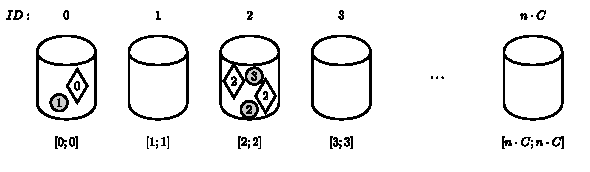
\includegraphics[width=\textwidth]{Chapter_II/SIMPLE-BUCKET-Example/a.pdf}
	\caption{ \textbf{Struktura oparta na kubełkach.} Pod każdym kubełkiem zaprezentowany jest indeks elementu tablicy, w~jakim się znajduje, oraz jego zakres. Do kubełka należą te węzły $v$, których $v.d$ znajduje się w zakresach, które są przypisane do każdego z kubełków (pomiędzy ,,$ \left[ \right]$''). } \label{fig:exampleSimpleBucket}
\end{figure}

Samo zaimplementowanie tablicy, indeksowanej od $0$ do $n \cdot C$ oczywiście nie zagwarantuje nam jeszcze poprawności działania algorytmu, polegającego na przeszukiwaniu (w~kolejności rosnących indeksów) elementów tablicy w~celu znalezienia węzła $v$ o~najmniejszej wartości etykiety $d$ i~zwróceniu go jako wynik operacji $\textrm{\textsc{EXTRACT-MIN}} \left( Q \right)$. Musimy rozważyć także sytuację, w~której dwa lub więcej węzłów w~trakcie działania algorytmu okazuje się być równoodległymi od źródła. Stąd pojawia się pojęcie \textbf{kubełków}, które będziemy traktować jako kontenery (najczęściej zaimplementowane jako listy dwukierunkowe) z~możliwymi operacjami $\textrm{\textsc{IS-EMPTY}} \left( B \right)$, $\textrm{\textsc{EXTRACT-HEAD}} \left( B \right)$, $\textrm{\textsc{EXTRACT-TAIL}} \left( B \right)$ oraz $\textrm{\textsc{EXTRACT-MIN}} \left( B \right)$, a które będą przechowywać wierzchołki grafu o~zadanych właściwościach. Właściwości kubełków będą różniły się w zależności od algorytmu~\cite[$79$--$81$]{GIDA}. W~tym przypadku będziemy mieli tablicę składającą się z~$n \cdot C + 1$ kubełków, gdzie każdy z~nich będzie mógł zawierać tylko takie węzły $v$, których $v.d = k$, gdzie $k$ to numer indeksu w~naszej tablicy (rysunek \ref{fig:exampleSimpleBucket}). 

Algorytm po kolei skanuje kubełki, poczynając od tego o~najniższym indeksie, wykonując relaksację dla napotkanych węzłów. W~naszym grafie nie ma krawędzi o~ujemnym koszcie (pokazaliśmy, że dla takiego przypadku algorytm Dijkstry nie działa), więc wykonując operację relaksacji dla dowolnego węzła $v_{i}$ w~kubełku o~indeksie $k$ ($v_{i}.d = k$) dla wszystkich krawędzi z~niego wychodzących $e : v_{i} \overset{1}\leadsto v_{j}$ , mamy pewność, że po jej wykonaniu dla każdego węzła $v_{j}$ zachodzi $v_{i}.d \leqslant v_{j}.d$. To zaś gwarantuje nam, że analizując kubełki w~takiej kolejności, jaką podaliśmy, nie pominiemy żadnego z~węzłów, należących do grafu $G$ (jeżeli tylko będą osiągalne ze źródła).

Algorytm działa w~czasie $ O \left( m + n \cdot C \right) $:

\begin{itemize}
\item W~najgorszym przypadku musimy przeskanować $ O \left( n \cdot C \right)$ kubełków,
\item Operację relaksacji w~najgorszym możliwym przypadku wykonamy za każdym razem, każdorazowo powodując przepięcie węzła $u$ z~jednego kubełka do drugiego (co między listami dwukierunkowymi zrobimy w~czasie stałym).
\end{itemize}

\subsection{Z przepełnieniem}

Jak nietrudno zauważyć, poprzednie podejście wykorzystywało ogromnie dużo pamięci, na dodatek nie zapewniając, że algorytm będzie działał dostatecznie szybko~--- stała $C$, którą ustalaliśmy na początku algorytmu, może być dowolnie duża, w~szczególności przekraczać $n$~--- otrzymalibyśmy wtedy algorytm nie tyle co o~dużej złożoności pamięciowej, ale także czasowej. W~tym podrozdziale postaramy się zaradzić pierwszemu z~problemów, ograniczając liczbę kubełków z~$n \cdot C$ do $a + 1$, gdzie za $a$ przyjmiemy dowolną liczbę mniejszą od $C + 1$. Dodatkowo wprowadzimy specjalny kubełek, do którego będą trafiać wszystkie takie węzły, których dystans do źródła będzie większy, niż zakres ostatniego z~$a$ kubełków. Innymi słowy ograniczymy ich liczbę z~pierwszego algorytmu, pozostawiając $a$ pierwszych kubełków, zaś wszystkie następne zastępując jednym, o~potencjalnie nieskończonym zakresie $ \left [ A~+ a~; \infty \right] $, gdzie początkowo $A = 0$. $\left( a + 1 \right)$'y kubełek będziemy nazywać przepełnieniem (ang. \textit{overflow bucket}).

\begin{pseudokod}[!htbp]
\DontPrintSemicolon
\Begin{
	$ \textrm{\textsc{INIT-GRAPH}} \left( G, s \right)$ \;
	\ForEach{$ i \in \left\{ 0 \cdots a~- 1 \right\} $}{
		$ B \left[ i \right] \longleftarrow \textrm{pusty kubełek o~zakresie } \left[ i~; i \right] $ \;
	}	
	$ B \left[ a \right] \longleftarrow \textrm{Overflow bag} $ \;
	
	\While{Wszystkie kubełki nie są puste} {
		\For{$i = 0$ \emph{\KwTo} $ a~- 1 $}{
			\ForEach{ $v_{j} \in B \left[ i \right] $}{
				Usuń $v_{j}$ z~$B \left[ i \right] $ \;
				\ForEach{$e_{jk} : v_{j} \overset{1} \leadsto v_{k}$}{
					$RELAX \left( v_{j}, v_{k} \right)$ \tcc*[f]{Jeśli $v_{k}.d$ się zmieniło, to przenieś $v_{k}$ do odpowiedniego kubełka.}\;
				}
			}
		}
		$ minDist \longleftarrow \min \left\{ v_{j}.d : v_{j} \in B \left[ a \right] \right\}$
		
		\ForEach{$ i \in \left\{ 0 \cdots a \right\} $}{
			$ B \left[ i \right] \longleftarrow \left[ minDist + i~; minDist + i \right] $ \tcc*[f]{Dla $B \left[ a \right]$ (\textit{overflow}) prawy zakres cały czas $ = \infty $)}\;
		}	
		\ForEach{ $v_{j} \in B \left[ a \right] $}{
			Przenieś $v_{j}$ do odpowiedniego kubełka. \;
		}
	}
}
\caption{ DKM $\left( G, s \right)$\label{alg:OverflowBucket}}
\end{pseudokod}

Algorytm rozpoczyna pracę od skanowania wszystkich kubełków, poczynając od tego o~najmniejszym zakresie. Dla kolejno napotkanych wierzchołków algorytm usuwa je, po czym wykonuje relaksacje dla wszystkich krawędzi z~nich wychodzących, odpowiednio aktualizując tablicę z~kubełkami. W~przypadku dojścia do ostatniego kubełka o~zakresie $ \left [ A~+ a~; \infty \right] $, algorytm wyszukuje w~nim najmniejszy (w sensie odległości od źródła) wierzchołek $v$ i~aktualizuje $A$, które jako wartość przyjmuje $v.d$. Następnie algorytm aktualizuje zakresy wszystkich pierwszych $a$ kubełków, których całkowity zakres wynosi $ \left [ A \left( i \right) ; A \left( i \right) + a~- 1 \right] $ w~$i$'tej iteracji algorytmu. Po przeniesieniu wszystkich wierzchołków do prawidłowych kubełków oraz zmianie ich zakresów, algorytm rozpoczyna kolejną iterację, wracając do pierwszego kubełka i~działa, dopóki wszystkie nie zostaną opróżnione (zob. pseudokod \ref{alg:OverflowBucket} oraz rysunek \ref{fig:exampleOverflowBucket}a--f)

\begin{figure}[!htbp]
	\centering
	\begin{subfigure}[b]{0.32\textwidth}
		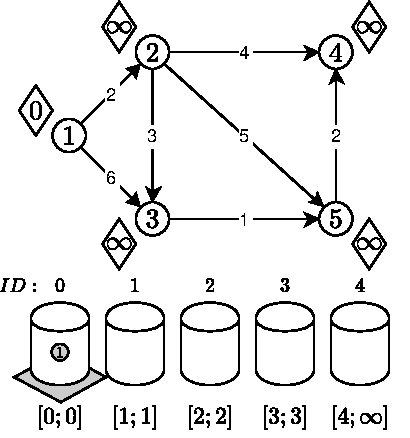
\includegraphics[width=\textwidth]{Chapter_II/OVERFLOW-BUCKET-Example/a.pdf}
		\caption{}
	\end{subfigure}%
	\begin{subfigure}[b]{0.32\textwidth}
		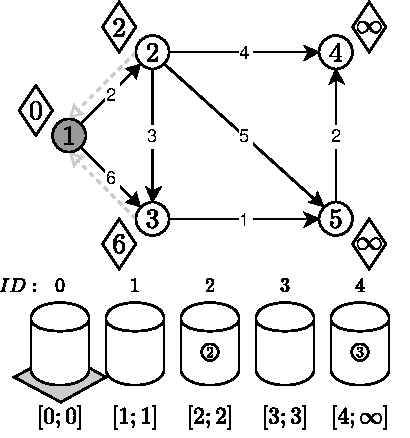
\includegraphics[width=\textwidth]{Chapter_II/OVERFLOW-BUCKET-Example/b.pdf}
		\caption{}
	\end{subfigure}
	\begin{subfigure}[b]{0.32\textwidth}
		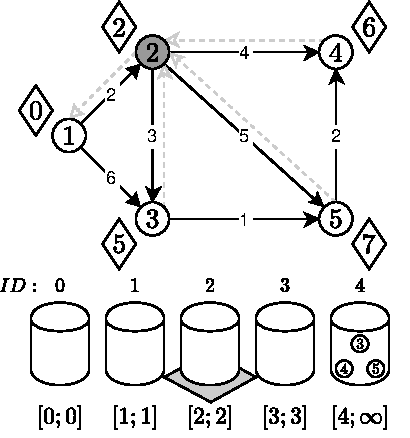
\includegraphics[width=\textwidth]{Chapter_II/OVERFLOW-BUCKET-Example/c.pdf}
		\caption{}
	\end{subfigure}
	\begin{subfigure}[b]{0.32\textwidth}
		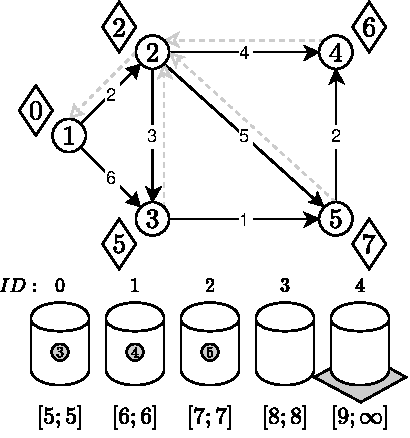
\includegraphics[width=\textwidth]{Chapter_II/OVERFLOW-BUCKET-Example/d.pdf}
		\caption{}
	\end{subfigure}%
	\begin{subfigure}[b]{0.32\textwidth}
		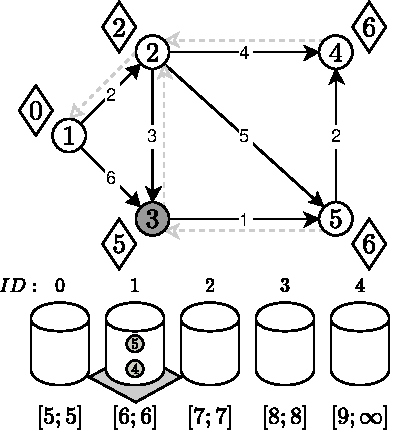
\includegraphics[width=\textwidth]{Chapter_II/OVERFLOW-BUCKET-Example/e.pdf}
		\caption{}
	\end{subfigure}
	\begin{subfigure}[b]{0.32\textwidth}
		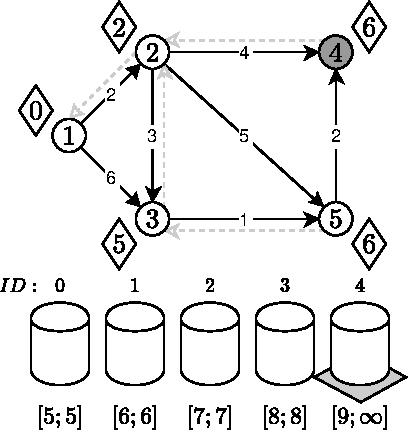
\includegraphics[width=\textwidth]{Chapter_II/OVERFLOW-BUCKET-Example/f.pdf}
		\caption{}
	\end{subfigure}
	\caption{\textbf{Działanie algorytmu DKM (alg. Dijkstry opartego na kubełkach z~przepełnieniem)} \textbf{(a)}  Sytuacja po zainicjowaniu grafu $G = \left( V, E \right)$ przez \textsf{INIT-GRAH} ze źródłem $v_{s}.id = 1$ i~$a = 4$. Badany kubełek jest na rysunku podświetlony zacieniowanym rombem. \textbf{(b)} Z~pierwszego kubełka został wyciągnięty jedyny wierzchołek. W~wyniku relaksacji krawędzi z~niego wychodzących do odpowiednich kubełków zostały dodane nowe węzły ($v_{2}.d = 2$ i~$ v_{2}.d \ni B \left[ 2 \right].range$ oraz $v_{3}.d = 6$ i~$ B \left[ a~- 1 \right].range < v_{3}.d $). \textbf{(c)} Kubełek $B \left[ 1 \right]$ był pusty. Algorytm wykonał operację \textsf{RELAX} dla następnego najmniejszego węzła: $v_{2}$ i~usunął go z~jego kubełka. W~jej wyniku zostały zrelaksowane krawędzie: $e_{24}$, $e_{23}$, i~$e_{25}$. Dla wszystkich węzłów $v$, wskazywanych przez te krawędzie, ich $v.d \in B \left[ a \right].range$. \textbf{(d)} Kubełek $B \left[ 3 \right]$ był pusty i~algorytm dotarł do ostatniego kubełka. Najmniejsza wartość $v.d$ dla $v \in B \left[ a \right]$ to $5$. Algorytm zaktualizował zakresy wszystkich kubełków i~przepiął wszystkie węzły z~badanego kubełka na ich odpowiednie miejsca. \textbf{(e)} Algorytm ponownie zaczął skanować kubełki od $B \left[ 0 \right]$ i~usunął z~niego węzeł $v_{3}$. W~wyniku relaksacji węzeł $v_{5}$ został przepięty do kubełka, odpowiadającego zakresem jego nowej odległości od źródła. \textbf{(f)} Po usunięciu z~kubełka $B \left[ 1 \right]$ węzłów $v_{4}$ i~$v_{5}$ (w dowolnej kolejności jako, że $v_{4}.d = v_{5}.d$) wszystkie kubełki są puste. } \label{fig:exampleOverflowBucket}
\end{figure}

\subsubsection{Złożoność obliczeniowa}

Algorytm działa w~czasie zależnym od parametru $a < C + 1$. Analizując zachowanie się algorytmu w~najgorszym możliwym przypadku mamy kolejno:

\begin{itemize}
\item $ O \left( \frac{n \cdot C}{a} \right) $~--- tyle razy zostaną przeskanowane wszystkie kubełki, gdzie w~każdej iteracji $i$ ich łączny zakres to $ \left [ A \left( i \right) ; A \left( i \right) + a~- 1 \right] $, nie licząc ostatniego węzła. Przed rozpoczęciem następnej iteracji algorytm zmienia zakresy wszystkich kubełków, wyszukując w~ostatnim z~nich węzeł $v$ taki, że $ v.d = \min \left\{ v_{i}.d : v_{i} \in B \left[ a \right] \right\}$, gdzie $v.d$ jest na pewno większe od prawej strony zakresu przedostatniego kubełka w~tablicy (wynika to z~samej własności zakresów kubełków, które są rozłączne). Niech zakres kubełka z~przepełnieniem podczas $i$'tej iteracji wynosi $ \left [ A \left( i \right) + a~; \infty \right] $.  W~najgorszym przypadku $v.d = A \left( i \right) + a$~--- wtedy podczas zmiany zakresów kubełków od $B \left[ 0 \right]$ do $B \left[ a~-1 \right]$ lewa strona nowego zakresu pierwszego kubełka jest o~$1$ większa od starego zakresu $B \left[ a~-1 \right]$. Dla tak zmienianych zakresów mamy zapewnione, że podczas  $\frac{n \cdot C}{a} $ iteracji każda wartość od $0$ do $n \cdot C - 1 $ będzie występowała jako zakres któregoś kubełka, nie będącego przepełnieniem, dokładnie jeden raz. W~najgorszym przypadku w~grafie będzie istnieć węzeł, którego odległość od źródła wynosi $ \left( n - 1 \right) \cdot C$, więc algorytm będzie musiał wykonać wszystkie $O \left( \frac{n \cdot C}{a} \right)$ iteracji, nim do niego dotrze i~usunie go z~kubełka.
\item Dla $a=C$ w~każdej kolejnej $i$'tej iteracji w~ostatnim kubełku znajduje się $k \left( i \right) $ węzłów, tak że $\cup _{i = 1}^{\frac{n \cdot C}{a}} \left| k \left( i \right) \right| = n - 1 $ (na przestrzeni działania całego algorytmu każdy z~$\left| V - 1 \right|$ wierzchołków, poza źródłem, znajdzie się w~tym kubełku dokładnie jeden raz). Łączny koszt wyszukiwania takiego węzła, że $ v.d = \min \left\{ v_{i}.d : v_{i} \in B \left[ a \right] \right\}$ we wszystkich iteracjach możemy zatem oszacować z~góry przez : $ O \left( n \right)$. Dla każdego innego $a$ własność ta może nie zachodzić, a oszacowanie wzrosnąć do $ O \left( n^{2} \right)$.
\item $ O \left( n \cdot C \right)$~--- w~takim czasie zostaną przeskanowane wszystkie kubełki, wyłączając kubełek ostatni, jeżeli algorytm wykona $ O \left( \frac{n \cdot C}{a} \right) $ iteracji (za każdym razem skanując $a+1$ kubełków).
\item Pod koniec każdej iteracji algorytm wykonuje przeniesienia wszystkich węzłów z~ostatniego kubełka~--- w~najgorszym możliwym przypadku takich wierzchołków będzie $ \sum_{i=1}^{\frac{n \cdot C}{a}} \left| v_{j} : v_{j} \in B \left[ a \right] \right| = O \left( n \right)$.
\item Poza przenoszeniem węzłów pod koniec każdej iteracji, algorytm wykonuje także $m$ relaksacji podczas skanowania pierwszych $a-1$ kubełków (w~trakcie trwania wszystkich rund).
\item Przeniesienie węzła z~kubełka $ B \left[ i \right] $ do $ B \left[ j \right]$ jest wykonywane w~czasie stałym.
\end{itemize}

W najgorszym możliwym przypadku algorytm może charakteryzować się złożonością $ O \left( n^{2} \right)$, która jest silnie zależna od operacji wyszukiwania minimum dla ostatniego kubełka.\label{DKMComplexity}

\subsection{Dial}

Zwróćmy uwagę, że dla $a=C$ poprzedni algorytm zachowuje się niemal identycznie, co opisany jako pierwszy (z $n \cdot C$ kubełkami), z~tą różnicą, że działa on w~rundach, gdzie maksymalnie może być ich $ O \left( \frac{n \cdot C}{a} \right) $. Pokazaliśmy, że dla tak dobranego parametru $a$ zakresy kubełków we wszystkich rundach tworzą \textbf{partycję}~\footnote{Rodzina niepustych, rozłącznych podzbiorów danego zbioru dająca w~sumie cały zbiór.}, taką że $\bigcup _{i=1}^{\frac{n \cdot C}{a}} \bigcup _{j=0}^{a-1} \left[ A \left( i \right ) + j ; A \left( i \right ) + j \right ] = \bigcup _{i=1}^{\frac{n \cdot C}{a}} \left[ A \left( i \right ) ; A \left( i \right ) + a~- 1 \right ] = \left[ 0 ; n \cdot C - 1 \right ]$, co sprowadza się do skanowania wszystkich kubełków o~zadanych zakresach z~naiwnej wersji algorytmu. Dopiero dla parametru $a < C$ możemy zacząć liczyć na to, że z~każdą iteracją pewna liczba kubełków zostanie pominięta. 

Wybór takiego ograniczenia dla $a$ ma swoje uzasadnienie i~wnioski, z~niego wynikające, zostały wykorzystane do usprawnienia następnego algorytmu, jakim jest algorytm wymyślony przez Roberta B. Diala~\cite[$4.6$]{Ahuja:1993:NFT:137406}, nazwany od nazwiska jego pomysłodawcy, którego pierwotna implementacja w~najgorszym przypadku także wymagała użycia $n \cdot C$ kubełków. W~wyniku modernizacji tego algorytmu ograniczono liczbę potrzebnych kubełków do $C+1$, powołując się na fakt, że w~żadnym momencie algorytmu, po wykonaniu relaksacji krawędzi, prowadzącej z~węzła $v_{i}$ do $v_{j}$ odległości od źródła tych dwóch węzłów są w~relacji: $v_{i}.d \leqslant v_{j}.d \leqslant v_{i}.d + C$, gdzie $C = \max \left\{ c_{ij} : e_{ij} \in E \right\}$. Wynika z~tego, że w~momencie skanowania $k$'tego kubełka spośród $C + 1$ kubełków i~założenia, że następnym kubełkiem po $B \left[ C \right] $ jest $B \left[ 0 \right] $, wszystkie węzły $v_{j}$, których odległość od źródła $v_{j}.d$ ulegnie zmianie w~wyniku relaksacji krawędzi wychodzących z~węzła $v_{i}$ (gdzie $v_{i}.d = k$), zostaną przemieszczone do kubełków o~indeksach od $k$ do $k + C$. Z~założenia, że kubełki ułożyliśmy na okręgu tak, by po ostatnim z~nich następował pierwszy, to indeks $k + C$ w~rzeczywistości odpowiada kubełkowi o~indeksie $ \left( k + C \right) \mod{C+1} = k - 1$. W~związku z~tym dla $C+1$ kubełków nigdy nie zajdzie sytuacja, by w~jednym kubełku znajdowały się węzły $v$ i~$u$, dla których $v.d \neq u.d$ (co oczywiście mogłoby się wydarzyć, gdybyśmy wzięli $c < C + 1$ kubełków).

\begin{figure}[!htbp]
	\centering
	\begin{subfigure}[b]{0.3\textwidth}
		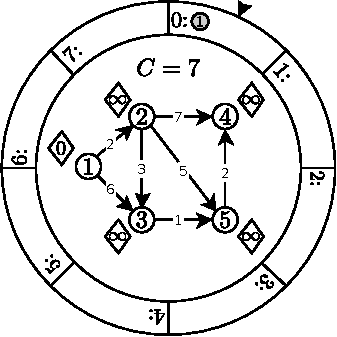
\includegraphics[width=\textwidth]{Chapter_II/DIAL-Example/a.pdf}
		\caption{}
	\end{subfigure}
	\qquad
	\begin{subfigure}[b]{0.3\textwidth}
		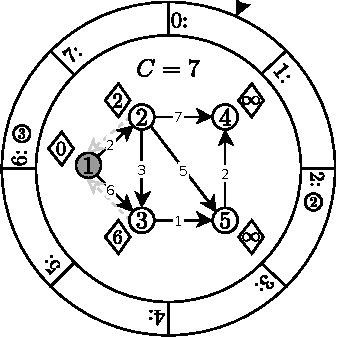
\includegraphics[width=\textwidth]{Chapter_II/DIAL-Example/b.pdf}
		\caption{}
	\end{subfigure}
	\qquad
	\begin{subfigure}[b]{0.3\textwidth}
		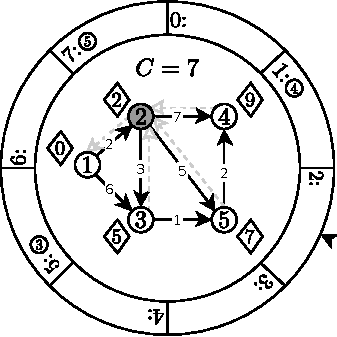
\includegraphics[width=\textwidth]{Chapter_II/DIAL-Example/c.pdf}
		\caption{}
	\end{subfigure}
	\qquad
	\begin{subfigure}[b]{0.3\textwidth}
		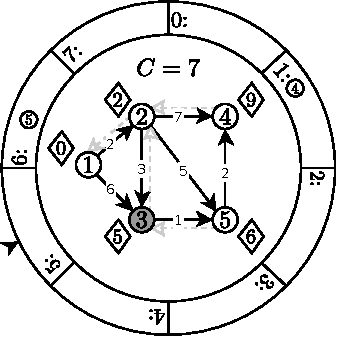
\includegraphics[width=\textwidth]{Chapter_II/DIAL-Example/d.pdf}
		\caption{}
	\end{subfigure}
	\qquad
	\begin{subfigure}[b]{0.3\textwidth}
		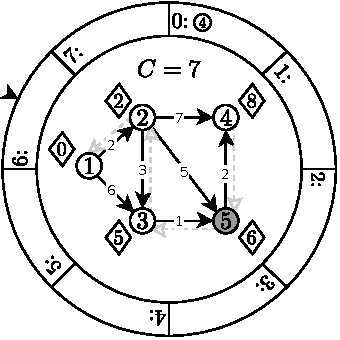
\includegraphics[width=\textwidth]{Chapter_II/DIAL-Example/e.pdf}
		\caption{}
	\end{subfigure}
	\qquad
	\begin{subfigure}[b]{0.3\textwidth}
		\includegraphics[width=\textwidth]{Chapter_II/DIAL-Example/f.pdf}
		\caption{}
	\end{subfigure}
	\caption{\textbf{Działanie algorytmu Dial z~$C+1$ kubełkami} \textbf{(a)} Sytuacja po zainicjowaniu grafu $G = \left( V, E \right)$ przez \textsf{INIT-GRAPH} ze źródłem $v_{s}.id = 1$. Mamy $C+1$ kubełków, indeksowanych od $0$ do $C$. Grot strzałki wskazuje obecnie badany kubełek. \textbf{(b)} Z~aktualnie badanego kubełka pobierany jest węzeł i~wykonywana jest relaksacje jego krawędzi wychodzących. W~jej wyniku do kubełków $B \left[ 2 \right]$ i~$B \left[ 6 \right]$ odpowiednio wstawione są węzły $v_{2}$ ($v_{2}.d = 2$) i~$v_{3}$ ($v_{3}.d = 6$). Następny kubełek ($B \left[ 1\right]$) jest pusty. \textbf{(c)} Algorytm przeskanował następny niepusty kubełek $B \left[ 2 \right]$, w~wyniku czego dokonał relaksacji krawędzi $e_{23}$, $e_{25}$ oraz $e_{24}$. Węzły na końcach tych krawędzi zmniejszyły swoją odległość od źródła $v_{1}$ i~zostały przeniesione do odpowiednich kubełków ($v_{4}.d = 9$, więc został przeniesiony do kubełka o~indeksie: $9 \mod{C+1} = 1$). \textbf{(d)} Następny niepusty kubełek to $B \left[ 5 \right]$, zawierający węzeł $v_{3}$ ($v_{3}.d = 5$), dla którego, w~wyniku relaksacji jego wychodzących krawędzi, przepięty zostaje węzeł $v_{5}$~--- jego odległość od węzła zmniejsza się z~$v_{5}.d = 7$ do $v_{5}.d = 6$. \textbf{(e)} Analogicznie jak w~poprzednim kroku, w~wyniku operacji \textsc{RELAX}, wykonanej dla krawędzi $e_{54}$, przepinany jest wierzchołek $v_{4}$ (z kubełka $B \left[ 9 \mod{C+1} \right]$ do $B \left[ 8 \mod{C+1} \right]$). \textbf{(f)} Algorytm skanuje następny niepusty kubełek, wykonuje potrzebne operacje relaksacji, po czym kończy działanie, jeżeli podczas całego jednego ,,obrotu''~ nie napotkał żadnego niepustego kubełka. } \label{fig:exampleDial}
\end{figure}

\subsubsection{Uwagi do algorytmu}

Jak w~każdym poprzednim przypadku, gdy zakres kubełków był jednostkowy (to znaczy $B \left[ i \right].range = \left[ k ; k \right]$), nie ważna jest kolejność wyciągania wierzchołków z~takiego kubełka. Co więcej, warto zauważyć, że dla pewnych sytuacji bardziej opłacalną operacją jest obliczanie nowych indeksów kubełków, do których mają trafić wierzchołki, w~czasie rzeczywistym, niż modyfikować już istniejące zakresy (w tym przypadku wykonywaliśmy operację $\mod{C+1}$, zamiast modyfikować zakresy wszystkich kubełków~--- przy omawianiu algorytmu opartego na kubełkach z~przepełnieniem taki indeks mogliśmy obliczyć, odejmując od $v.d$, dla dowolnego $v$, wyrażenie $A \left( i \right)$). Analizując obydwa podejścia mamy następującą sytuację:

\begin{center}
	\begin{tabular}{ccc}
		& Liczba iteracji & Złożoność obliczeniowa pojedynczego wywołania \\
		\hline
		Zmiana zakresu kubełków & $ O \left( n \right) $ & $ \Theta \left( C + 1 \right) $ \\
		Modulowanie indeksów & $ \Theta \left( m \right) $ & $ \Theta \left( 1 \right) $ \\
		\hline
	\end{tabular}
\end{center}

W pierwszym przypadku liczba modyfikacji zakresów każdego z~$C+1$ kubełków jest ściśle zależna od liczby ,,okrążeń''~, jakie musi wykonać algorytm Dijkstry, by przeskanować wszystkie wierzchołki w~grafie. Dla drugiego przypadku liczba operacji obliczania nowych indeksów wierzchołków jest ściśle ograniczona do liczby wykonywanych relaksacji na przestrzeni działania całego algorytmu. Zastosowanie pierwszego wariantu dodatkowo wymaga od nas stworzenia osobnej struktury, która umożliwiałaby przechowywanie zakresów każdego z~$C+1$ kubełków (gdyż, w~przypadku algorytmu Dial, podstawą do obliczenia zakresów kubełków są ich indeksy w~tablicy $ B \left[ 0 \cdots C \right]$).

Na sam koniec możemy zauważyć, że warunek, który musi zajść, by algorytm Dial zakończył działanie (to jest w~momencie, gdy wszystkie kubełki są puste) wymaga od nas wykonania $ O \left( n \cdot C \right)$ operacji (w najgorszym przypadku), podczas gdy możemy zastąpić je przez sprawdzanie, czy w~momencie wykonywania relaksacji węzeł, którego odległość od źródła się zmienia, zostanie przeniesiony do kubełka o~mniejszym indeksie niż ten, który aktualnie skanujemy. Jeżeli taka sytuacja nie będzie miała miejsca dla żadnego ze skanowanych $C+1$ kubełków, to znaczy, że wszystkie kubełki są puste i~po wykonaniu skanowania ostatniego kubełka algorytm powinien zakończyć pracę. Jednak, tak jak w~poprzednim przypadku, jest to tylko niewielka modyfikacja, zamieniająca złożoność jednej ze składowych operacji algorytmu Dijkstry z~$ O \left( n \cdot C \right)$ na $ O \left( m \right)$ i~na odwrót.

\subsubsection{Złożoność obliczeniowa}

Algorytm Dial działa w~czasie $O \left( m + n \cdot C \right)$~--- algorytm wykona co najwyżej $m$ operacji relaksacji, każdą w~czasie $O \left( 1 \right)$, i~będzie musiał przeskanować, w~najgorszym przypadku, $O \left( n \cdot C \right)$ kubełków.


\subsection{Aproksymacja zakresu}

W poprzednich algorytmach skupialiśmy się na redukcji liczby wykorzystywanych kubełków w~celu oszczędzenia jak największej części pamięci operacyjnej i~przyspieszeniu obliczeń, zachowując jednocześnie jednostkowe zakresy kubełków, co w~najgorszych przypadkach zmuszało nas do wykonania $O \left( n \cdot C \right)$ operacji bez względu na to, jak przeglądaliśmy stworzone przez nas kubełki, bez względu na ich strukturę. Przedstawiony poniżej algorytm jest pierwszym algorytmem typu korekcyjnego (ang. \textit{Label Correcting Algorithm}~\cite[$2.4$]{OR}), opartym na kubełkach. Algorytmy tego typu różnią się od do tej pory omawianych ( $LSA$~--- ang. \textit{Label Setting Algorithm}~\cite[$2.1$]{OR}) tym, że nie posiadają własności, zapewniającej nas o~zajściu warunku $v.d = \delta \left( s, v \right)$ tuż po wykonaniu relaksacji dla wszystkich krawędzi, wychodzących z~tego wierzchołka i~usunięciu go z~listy wierzchołków, czekających na przetworzenie~\cite[$17$]{OR}. Innymi słowy dopuszczamy w~nich możliwość wielokrotnego poprawiania odległości od źródła dla dowolnego węzła, bez zachowania kolejności ich poprawiania w~porządku (zob. pseudokod \ref{alg:GenericLabelCorrectingAlgorithm}), jaki wcześniej zapewniały nam kolejki priorytetowe (algorytm Bellmana-Forda jest też takim algorytmem). 

\begin{pseudokod}[!htbp]
\DontPrintSemicolon
\Begin{
	$ \textrm{\textsc{INIT-GRAPH}} \left( G, s \right)$ \;
	\While{$ \exists e_{ij} : v_{i} \overset{1} \leadsto v_{j} \; \wedge \; v_{j}.d > v_{i}.d + c_{ij} $} {
		$RELAX \left( v_{i}, v_{j} \right)$ \;
	}
}
\caption{ GENERIC-LABEL-CORRECTING-ALGORITHM $\left( G, s \right)$\label{alg:GenericLabelCorrectingAlgorithm}}
\end{pseudokod}

\newpage
\begin{proof}

Bardzo łatwo wykazać, że powyższy algorytm działa w~skończonym czasie i~zwraca poprawne wyniki. Wiemy, że dla każdego węzła $v$ po inicjalizacji grafu procedurą $ \textrm{\textsc{INIT-GRAPH}} \left( G, s \right)$ zachodzi $v.d \geqslant \delta \left( s, v \right)$ a~dodatkowo $n \cdot C \geqslant v.d$. Dla grafu z~ujemnymi kosztami ścieżek, z~którymi algorytm typu $LCA$ jest w~stanie sobie poradzić, możemy także dopisać $ \delta \left( s, v \right) > - n \cdot C$. Dla każdego znalezionego łuku $e_{ij}$ w~grafie, takiego że zachodzi $v_{j}.d > v_{i}.d + c_{ij}$ algorytm wykonuje relaksację, po której $v_{j}.d = v_{i}.d + c_{ij}$~--- inaczej mówiąc podczas każdej relaksacji zmniejsza wartość $v_{j}.d$ co najmniej o~$1$. Z~ograniczenia $ n \cdot C \geqslant v_{j}.d \geqslant \delta \left( s, v_{j} \right) > - n \cdot C$ wynika zatem, że w~najgorszym przypadku algorytm potrzebuje wykonać $2 \cdot n \cdot C$ kroków, by $v_{j}.d \leqslant v_{i}.d + c_{ij}$ dla każdego węzła $v_{i}$ (dla $v_{j}.d = \delta \left( s, v_{j} \right)$ z~lematu \ref{lem:costUpperBound}). Analogicznie wykonamy operacje relaksacji dla wszystkich $n$ węzłów w~grafie, więc po $O \left( n \cdot \left( n \cdot C \right) \right) $ krokach algorytm zakończy działanie i~dla wszystkich węzłów $v$: $v.d = \delta \left( s, v \right)$.

\end{proof}

W algorytmie, wykorzystującym aproksymacyjne kubełki (ang. \textit{Dijkstra algorithm with implemented with approximate buckets}), zakres każdego $i$'tego kubełka określany jest jako $ \left[ i \cdot b ; \left( i~+ 1 \right) \cdot b - 1 \right]$, gdzie $b < C + 1$. Algorytm łączy w~sobie ideę konieczności posiadania jedynie $C+1$ kubełków, dodatkowo jeszcze zmniejszając ich liczbę, poszerzając ich zakresy, co powoduje, że potrzebujemy ich już tylko $\left \lfloor \frac{C}{b} \right \rfloor + 1$ (zob. pseudokod \ref{alg:AproximateBuckets}). Wierzchołki w~każdym kubełku są trzymane w~kolejce $FIFO$ (nie przejmujemy się kolejnością wyciągania wierzchołków w~przypadku, gdy jest ich kilka w~jednym kubełku), a~ich skanowanie odbywa się na dokładnie tej samej zasadzie co w pozostałych algorytmach tego typu~\cite[$23$--$24$]{Dissertation}.

\begin{pseudokod}[!htbp]
\DontPrintSemicolon
\Begin{
	$ \textrm{\textsc{INIT-GRAPH}} \left( G, s \right)$ \;
	$ K \longleftarrow \left \lfloor \frac{C}{b} \right \rfloor + 1$ \;
	\ForEach{$ i \in \left\{ 0 \cdots K \right\} $}{
		$ B \left[ i \right] \longleftarrow \textrm{pusty kubełek o~zakresie } \left[ i \cdot b ; \left( i~+ 1 \right) \cdot b - 1 \right] $ \;
	}	
	
	\While{Wszystkie kubełki nie są puste} {
		\For{$i = 0$ \emph{\KwTo} $ K $}{
			\ForEach{ $v_{j} \in B \left[ i \right] $}{
				Usuń $v_{j}$ z~$B \left[ i \right] $ \;
				\ForEach{$e_{jk} : v_{j} \overset{1} \leadsto v_{k}$}{
					$RELAX \left( v_{j}, v_{k} \right)$ \tcc*[f]{Jeśli $v_{k}.d$ się zmieniło, to przenieś $v_{k}$ do odpowiedniego kubełka.}\;
				}
			}
		}
	}
}
\caption{ DKA $\left( G, s \right)$\label{alg:AproximateBuckets}}
\end{pseudokod}

\subsubsection{Złożoność obliczeniowa}

W najgorszym przypadku algorytm działa w~czasie $ O \left( m \cdot b + n \cdot \left( b + \frac{C}{b}\right) \right)$:

\begin{itemize}
\item Tak jak w~każdym przypadku, gdy mieliśmy do czynienia ze strukturą opartą na kubełkach, algorytm, by skończyć działanie, musi je wszystkie przeglądnąć. W~najgorszym przypadku dla każdego z $n$ węzłów będziemy musieli przenosić je do kubełków o coraz niższych indeksach~--- tych mamy $O \left( \frac{C}{b} \right)$, co łącznie daje nam czas, ograniczony z~góry przez: $O \left( n \cdot \frac{C}{b} \right)$.
\item Przyjrzyjmy się sytuacji, w~której do kubełka $k$ o~zakresie $\left[ i \cdot b ; \left( i~+ 1 \right) \cdot b - 1 \right]$ pierwszy raz jest wstawiany węzeł $v_{j}$ taki, że $v_{j}.d = \left( i~+ 1 \right) \cdot b - 1$. Przyjmijmy dodatkowo, że dla każdej relaksacji krawędzi, która prowadzi do tego węzła odległość $v_{j}.d$ jest zmniejszana o~$1$ tak, że jest on $b$ razy wstawiany do tego samego kubełka. W~takim przypadku algorytm, w~wyniku skanowania kubełka $k$, wyciągnie dany wierzchołek dokładnie $b$ razy, gdzie za ostatnim razem wierzchołek znajduje się na samym początku kubełka ($v_{j}.d = i \cdot b$). W~czasie skanowania kubełka relaksacje (w liczbie $k$), które są wykonywane, dotyczą tylko takich krawędzi $e : v_{l} \overset{1}\leadsto v_{j}$, dla których węzły $v_{l} \in B \left[ k \right]$, z~czego wynika, że dla dowolnego takiego wierzchołka $ i \cdot b \leqslant v_{l}.d \leqslant \left( i~+ 1 \right) \cdot b - 1$. Zatem, gdy $v_{j}.d = i \cdot b$ to dla dowolnej operacji $RELAX \left( v_{l}, v_{j} \right)$ będziemy mieli $ v_{j}.d \geqslant v_{l} + c_{lj} = i \cdot b \geqslant i \cdot b + c_{lj}$ (dla kosztów ścieżek nieujemnych), co jest równoważne temu, że relaksacja krawędzi nigdy już nie zajdzie, a~tym samym nie dodamy wierzchołka $v_{j}$ ponownie do któregoś z~kubełków (algorytm skanuje kubełki od lewej do prawej, więc relaksacja, którą opisaliśmy, tym bardziej nie zajdzie, jeżeli pójdziemy do dalszych kubełków). W~związku z~tym dany  wierzchołek algorytm będzie badał co najwyżej $b$ razy. Dla $n$ wierzchołków mamy ograniczenie $O \left( n \cdot b \right)$.
\item Bezpośrednio z~powyższego wniosku wynika także, że algorytm może w~najgorszym przypadku wykonać $O \left( m \cdot b \right)$ relaksacji (dla każdego kubełka $b$ razy).
\end{itemize}

Ostatecznie daje nam to złożoność algorytmu, ograniczoną z~góry przez $ O \left( m \cdot b + n \cdot \left( b + \frac{C}{b}\right)\right)$. Warto zwrócić uwagę, że dla $b=1$ (czyli, gdy kubełki mają jednostkowe zakresy) otrzymujemy algorytm Dial, którego złożoność wynosiła $ O \left( m + n \cdot C \right)$.

\begin{figure}[!htbp]
	\centering
	\begin{subfigure}[b]{0.42\textwidth}
		\includegraphics[width=\textwidth]{Chapter_II/APROXIMATE-BUCKETS-Other/sparseGraphPlot3D_psfrag.pdf}
		\caption{}
	\end{subfigure}
	\qquad
	\begin{subfigure}[b]{0.42\textwidth}
		\includegraphics[width=\textwidth]{Chapter_II/APROXIMATE-BUCKETS-Other/fullGraph3DPlot_psfrag.pdf}
		\caption{}
	\end{subfigure}
	\caption{\textbf{Wykresy zależności $ O \left( m \cdot b + n \cdot \left( b + \frac{C}{b} \right) \right) $ dla $C = 10000$ } \textbf{(a)} Wykres przedstawia zależność czasu działania algorytmu od liczby węzłów i~szerokości kubełków dla grafu rzadkiego ($ m = n $). \textbf{(b)} Wykres przedstawia zależność czasu działania algorytmu od liczby węzłów i~szerokości kubełków dla grafu pełnego ($ m = \frac{n \cdot \left( n - 1\right)}{2}$). Wyraźnie widzimy, że algorytm zamienia złożoność obliczeniową na pamięciową (i odwrotnie). }\label{fig:plotAproximateBucketsComplexity}
\end{figure}

\begin{figure}[!htbp]
	\centering
	\begin{subfigure}[b]{0.27\textwidth}
		\includegraphics[width=\textwidth]{Chapter_II/APROXIMATE-BUCKETS-Example/a.pdf}
		\caption{}
	\end{subfigure}%
	\begin{subfigure}[b]{0.27\textwidth}
		\includegraphics[width=\textwidth]{Chapter_II/APROXIMATE-BUCKETS-Example/b.pdf}
		\caption{}
	\end{subfigure}
	\begin{subfigure}[b]{0.27\textwidth}
		\includegraphics[width=\textwidth]{Chapter_II/APROXIMATE-BUCKETS-Example/c.pdf}
		\caption{}
	\end{subfigure}
	\caption{\textbf{Działanie algorytmu Dijkstry, opartego na aproksymacji kubełków} \textbf{(a)} Początkowa sytuacja w~grafie $G$ ($b=2$). \textbf{(b)} Z~pierwszego, przeskanowanego kubełka został wyciągnięty węzeł $v_{1}$. W~wyniku relaksacji do kubełków $B \left[ 1 \right]$ i~$B \left[ 3 \right]$ odpowiednio zostały włożone węzły: $v_{2}$ i~$v_{3}$.  \textbf{(c)} Po wykonaniu relaksacji $B \left[ 0 \right]$ jest pusty~--- algorytm rozpoczął skanowanie kubełka $B \left[ 1 \right]$, po czym wyciągnął z~niego wierzchołek $v_{2}$, wykonując następnie relaksacje krawędzi z~niego wychodzących. } \label{fig:exampleAproximateBuckets1}
\end{figure}

\begin{figure}[!htbp]
	\ContinuedFloat
	\centering
	\begin{subfigure}[b]{0.3\textwidth}
		\includegraphics[width=\textwidth]{Chapter_II/APROXIMATE-BUCKETS-Example/d.pdf}
		\caption{}
	\end{subfigure}%
	\begin{subfigure}[b]{0.3\textwidth}
		\includegraphics[width=\textwidth]{Chapter_II/APROXIMATE-BUCKETS-Example/e.pdf}
		\caption{}
	\end{subfigure}
	\begin{subfigure}[b]{0.3\textwidth}
		\includegraphics[width=\textwidth]{Chapter_II/APROXIMATE-BUCKETS-Example/f.pdf}
		\caption{}
	\end{subfigure}
	\caption{ \textbf{(d)} Po wykonaniu relaksacji dla wszystkich wierzchołków $v \in B \left[ 1 \right]$, algorytm rozpoczyna skanowanie następnego kubełka w~tablicy. Dla wierzchołka $v_{3} \in B \left[ 2 \right]$ wykonana jest relaksacja krawędzi $e_{35}$ a~następnie~--- dla pustego już kubełka~--- algorytm przechodzi do kolejnego. \textbf{(e--f)} Z~kubełka $ B \left[ 3 \right]$ kolejno są wyciągane węzły. Algorytm przeprowadza ostatnie relaksacje i~kończy działanie.} \label{fig:exampleAproximateBuckets2}
\end{figure}

\subsection{Kubełki wielopoziomowe}

Kolejnym algorytmem, któremu poświęcimy naszą uwagę, będzie algorytm oparty na kubełkach wielopoziomowych (w naszym przypadku będą to da poziomy~\cite[$4.2$]{NetOpt}). Dotychczasowe algorytmy, które były oparte o~tą strukturę danych, wykorzystywały model jednopoziomowy, w~różny sposób podchodząc do jego implementacji. W~tym algorytmie zamiast jednego poziomu kubełków, który wcześniej zwykliśmy oznaczać przez $B \left[ 0 \cdots k \right]$, będziemy wykorzystywać oznaczenia $B_{\mathbb{L}} \left[ 0 \cdots k_{\mathbb{L}} \right]$ i~$B_{\mathbb{U}} \left[ 0 \cdots k_{\mathbb{U}} \right]$ odpowiednio dla kubełków niskiego (ang. \textit{Low-level buckets}) oraz wysokiego poziomu (ang. \textit{High-level buckets}). Ideą algorytmu jest stworzenie $ \left \lfloor \frac{n \cdot C}{d} \right \rfloor $ kubełków wysokiego poziomu, gdzie każdy $i$'ty taki kubełek ma zakres $ \left[ i \cdot d ; \left( i+1 \right) \cdot d - 1\right]$ oraz $d$ kubełków niskiego poziomu o~zakresach jednostkowych~--- tym samym suma ich zakresów wynosi dokładnie $ \left[ L \cdot d ; \left( L+1 \right) \cdot d - 1\right]$ (początkowo $L=0$). W~czasie pracy algorytm nieprzerwanie skanuje kubełki o~zakresach jednostkowych od lewej do prawej. Gdy wszystkie wierzchołki z~kubełków niskiego poziomu zostaną usunięte, algorytm wyszukuje pierwszy niepusty kubełek $k \in B_{\mathbb{U}}$, odpowiednio zwiększa $L$ a~następnie przenosi wszystkie wierzchołki $v \in k$ do odpowiednich kubełków niskiego poziomu, rozpoczynając ich skanowanie od początku. Algorytm wykonuje pracę, dopóki na którejś z~list znajdują się nieprzetworzone wierzchołki. Algorytm powstał jako złączenie dwóch poprzednich: w~oparciu o~kubełki z~przepełnieniem oraz algorytm $DKA$ (szczególnie do tego ostatniego widzimy podobieństwo z~sposobie implementacji kubełków wysokiego poziomu).

\begin{figure}[!htbp]
	\centering
	\begin{subfigure}[b]{0.45\textwidth}
		\includegraphics[width=\textwidth]{Chapter_II/DOUBLE-LEVEL-BUCKET-Example/a.pdf}
		\caption{}
	\end{subfigure}%
	\caption{\textbf{Działanie algorytmu $DKD$} \textbf{(a)} Sytuacja po zainicjowaniu grafu $G$ ($d=4$, $n \cdot C = 15$). Do pierwszego kubełka w~$B_{\mathbb{L}}$ wstawiony zostaje wierzchołek, będący źródłem. } \label{fig:exampleDoubleLevelBuckets1}
\end{figure}
	
\begin{figure}[!htbp]
	\ContinuedFloat
	\centering
	\begin{subfigure}[b]{0.45\textwidth}
		\includegraphics[width=\textwidth]{Chapter_II/DOUBLE-LEVEL-BUCKET-Example/b.pdf}
		\caption{}
	\end{subfigure}%
	\qquad
	\begin{subfigure}[b]{0.45\textwidth}
		\includegraphics[width=\textwidth]{Chapter_II/DOUBLE-LEVEL-BUCKET-Example/c.pdf}
		\caption{}
	\end{subfigure}
	\begin{subfigure}[b]{0.45\textwidth}
		\includegraphics[width=\textwidth]{Chapter_II/DOUBLE-LEVEL-BUCKET-Example/d.pdf}
		\caption{}
	\end{subfigure}%
	\qquad
	\begin{subfigure}[b]{0.45\textwidth}
		\includegraphics[width=\textwidth]{Chapter_II/DOUBLE-LEVEL-BUCKET-Example/e.pdf}
		\caption{}
	\end{subfigure}
	\begin{subfigure}[b]{0.45\textwidth}
		\includegraphics[width=\textwidth]{Chapter_II/DOUBLE-LEVEL-BUCKET-Example/f.pdf}
		\caption{}
	\end{subfigure}
	\qquad
	\begin{subfigure}[b]{0.45\textwidth}
		\includegraphics[width=\textwidth]{Chapter_II/DOUBLE-LEVEL-BUCKET-Example/g.pdf}
		\caption{}
	\end{subfigure}%
	\caption{ \textbf{(b)} Algorytm rozpoczyna skanowanie kubełków niskiego poziomu (aktualny postęp algorytmu dla obu poziomów jest zaznaczony za pomocą rombów pod odpowiednimi kubełkami). Algorytm wykonuje relaksację dla wszystkich krawędzi $e : v_{1} \overset{1}\leadsto v_{i}$, w~wyniku której do kubełka $K_{\mathbb{L}} \left[ 2\right]$ wstawione zostają węzły $v_{2}$ oraz $v_{3}$ ($v_{2}.d = v_{3}.d = 2$). \textbf{(c)} Algorytm zatrzymuje się na pierwszym niepustym kubełku, wyjmując z~niego dowolny element (na rysunku $v_{2}$) oraz przeprowadzając relaksacje jego wychodzących krawędzi ($e_{23}$, $e_{24}$ i~$e_{25}$). W~ich wyniku węzły $v_{4}$ oraz $v_{5}$ stały się osiągalne ze źródła i~zostały wstawione do kubełka $K_{\mathbb{U}} \left[ 0 \right]$ ($v_{4}.d, v_{5}.d \in K_{\mathbb{U}} \left[ 0 \right].range$). \textbf{(d)} W~wyniku relaksacji krawędzi wychodzących z~aktualnie badanego węzła $v_{3}$, dla wierzchołka $v_{5}$ została zmniejszona odległość od źródła tak, że $v_{5}.d \leqslant K_{\mathbb{L}} \left[ d - 1 \right].range$. Wierzchołek został z~powrotem przepięty do tablicy kubełków niskiego poziomu, do kubełka $K_{\mathbb{L}} \left[ 3 \right]$. \textbf{(e)} Z~ostatniego niepustego kubełka został wyjęty węzeł $v_{5}$. Po przeprowadzeniu operacji \textsc{RELAX} wszystkie kubełki $k \in K_{\mathbb{L}}$ są puste. Algorytm kontynuuje skanowanie kubełków wysokiego poziomu, zatrzymując się na pierwszym niepustym. \textbf{(f)} Następuje zmiana zakresów kubełków dolnego poziomu (tak, że zachodzi $ \left[ K_{\mathbb{L}} \left[ 0 \right].lrange ; K_{\mathbb{L}} \left[ d - 1 \right].rrange \right] = K_{\mathbb{U}} \left[ 0 \right].range$), a~następnie wszystkie wierzchołki z~kubełka $K_{\mathbb{U}} \left[ 0 \right]$ zostają przeniesione do odpowiednich kubełków w~tablicy $K_{\mathbb{L}}$. Po przeniesieniu wszystkich węzłów, algorytm rozpoczyna na nowo skanowanie kubełków $K_{\mathbb{L}} \left[ 0 \cdots d-1 \right]$. \textbf{(g)} Z~kubełka $K_{\mathbb{L}} \left[ 0 \right]$ zostaje wyjęty ostatni wierzchołek. Po wykonaniu relaksacji dla krawędzi wychodzących z~$v_{4}$ (brak jest takich), wszystkie kubełki są puste. Algorytm, doszedłszy do końca $B_{\mathbb{U}}$, kończy pracę.} \label{fig:exampleDoubleLevelBuckets2}
\end{figure}

\subsubsection{Złożoność obliczeniowa~--- kubełki 2-poziomowe}

Analizując złożoność obliczeniową algorytmu Dijkstry, opartego o~kubełki wielopoziomowe, podzielimy naszą analizę na dwie części: w~pierwszej z~nich pokażemy złożoność algorytmu, którego przykład przedstawiono na rysunku \ref{fig:exampleDoubleLevelBuckets1}, zaś następnie uogólnimy algorytm na $k$ poziomów.

Algorytm oparty na kubełkach dwupoziomowych składa się z~trzech faz, którymi są: skanowanie górnej części kubełków, przenoszenie wierzchołków do tablicy $B_{\mathbb{L}} \left[ 0 \cdots d-1 \right]$ oraz wykonywanie skanowania kubełków niskiego poziomu w~celu wykonania relaksacji dla krawędzi wychodzących z~wierzchołków, które tam się znajdą. Kolejno mamy zatem:

\begin{itemize}
\item $O \left( \frac{n \cdot C}{d} \right)$~--- jest to czas potrzebny na przeskanowanie kubełków wysokiego poziomu, których jest $ \left \lfloor \right \frac{n \cdot C}{d} \rfloor $. W~najgorszym przypadku będziemy musieli przeskanować je wszystkie.
\item Bez względu na to, ile kubełków wysokiego poziomu przeskanowaliśmy, co najwyżej $ \left| V \right|$ wierzchołków zostanie przeniesionych z~$B_{\mathbb{U}} \left[ 0 \cdots \left \lfloor \frac{n \cdot C}{d} \right \rfloor -1 \right]$ do $B_{\mathbb{L}} \left[ 0 \cdots d-1 \right]$, a~zatem w~najgorszym możliwym przypadku będziemy zmuszeni do wykonania $ \left| V \right|$ skanowań kubełków niskiego poziomu, za każdym razem skanując ich $d$, gdzie na skanowanie jednego kubełka przypada $O \left( 1 \right)$. Zatem łączny kosz tej operacji to $O \left( n \cdot d \right)$.
\item W~omawianym powyżej przypadku algorytm będzie musiał $n = \left| V \right|$ razy wykonać zmiany zakresów każdego z~$d-1$ kubełków. Wykorzystując fakt, że zakres każdego z~kubełków jest opisany w~zależności od jednej zmiennej $L$ ($B_{\mathbb{L}} \left[ i \right].range =  \left[ L \cdot d + i~; \left( L+1 \right) \cdot + i \right]$), gdzie $L$ oznacza najmniejszą wartość zakresu aktualnie badanego kubełka wysokiego poziomu, jesteśmy w~stanie przeprowadzić taką zmianę w~czasie stałym (obliczenia związane z~wstawianiem wierzchołka do odpowiedniego kubełka zostaną wykonane każdorazowo w~czasie $O \left( 1 \right)$ i~są zależne od liczby przemieszczanych z~$B_{\mathbb{U}}$ do $B_{\mathbb{L}}$ wierzchołków ~--- maksymalnie $n$).
\item Ostatnią fazą algorytmu, jaką wyodrębniliśmy, była faza relaksacji wierzchołków, a~tych jest co najwyżej $m$~--- każdy wierzchołek, będący w~kubełkach niskiego poziomu, skanujemy dokładnie raz.
\end{itemize}

Podsumowując powyższe rozważania: algorytm Dijkstry, zbudowany w~oparciu o~strukturę kubełków dwupoziomowych, działa w~czasie nieprzekraczającym $ O \left( \frac{n \cdot C}{d} + n \cdot d + m \right)$. Tak jak w~przypadku, gdy analizowaliśmy algorytm oparty na kopcach $R$-arnych, tak samo tutaj zoptymalizowany czas działania algorytmu otrzymamy, gdy doprowadzimy największe wyrażenia, od których zależy ten czas, do równości (czyli do: $\frac{n \cdot C}{d} = n \cdot d$), z~której natychmiastowo wynika $d = \sqrt{C}$.

Warto też zwrócić uwagę na to, że naiwna implementacja, którą zajmowaliśmy się na samym początku to tak naprawdę algorytmy jednopoziomowe, dla których poniższa analiza jest jak najbardziej prawidłowa ($ O \left( \frac{n \cdot C}{1} + n \cdot 1 + m \right) = O \left( m + n \cdot C \right)$). Nasuwa się pytanie, czy takiej samej analizy nie możemy przeprowadzić dla algorytmu Dial, który także jest implementacją jednopoziomową (jego kubełki mają identyczne własności co $B_{\mathbb{L}}$). Odpowiedź oczywiście jest pozytywna.

Niech maksymalna liczba kubełków wysokiego poziomu wynosi $\left \lfloor \frac{C+1}{d} \right \rfloor$ i~niech dodatkowo $d = \sqrt{C + 1}$ ($C+1$ kubełków wymagała implementacja algorytmu Dial). Zauważmy, że w~takiej sytuacji mamy tyle samo kubełków na każdym poziomie a~każdy z~$ \sqrt{C + 1}$ ma ten sam zakres, gdzie dla $i$'tego kubełka wynosi on $ \left[ i \cdot d ; \left( i+1 \right) \cdot d - 1\right]$. Łącznie daje to nam rozpiętość kubełków: $ \left[ 0 ; \left( \sqrt{C + 1} +1 \right) \cdot \sqrt {C + 1} - 1\right] = \left[ 0 ; \left( C + 1 \right) + \sqrt{C + 1} - 1 \right] $ (dla przypadku algorytmu Dial wymagany zakres kubełków to $ \left[ 0 ; C \right]$). Wykonując teraz analizę okaże się, że otrzymamy takie samo oszacowanie na złożoność obliczeniową, co dla przypadku, gdy $ \left| B_{\mathbb{U}} \right| = \left \lfloor \frac{n \cdot C}{d} \right \rfloor $, gdzie $d = \sqrt{C}$ (a zatem $ O \left( \frac{n \cdot C}{d} + n \cdot d + m \right) =  O \left( n \cdot \sqrt{C} + m \right)$).

Podstawową naszą obserwacją będzie fakt, że algorytm do pracy wymaga $ 2 \cdot \sqrt{C+1}$ kubełków. Jak przekonaliśmy się podczas poprzedniej analizy, każdy z~kubełków wysokiego poziomu może zostać zbadany co najwyżej raz i~taką samą liczbę razy, jak wcześniej, może być wymagane wykonanie skanowania dla wszystkich kubełków niskiego poziomu, wraz ze zmianą ich zakresów w czasie stałym ($n \cdot \sqrt{C+1}$ i $n \cdot 1$). Dodatkowo może być wymagane przeskanowanie każdego kubełka należącego do $K_{\mathbb{U}}$ w~celu zakończenia pracy algorytmu ($ \sqrt{C+1}$). Daje nam to łącznie złożoność, ograniczoną przez $ O \left( m + n \cdot \left( 1 + \sqrt{C} \right) \right)$ (relaksacji jak zawsze potrzebujemy wykonać najwyżej $m$), co daje nam $O \left( n \cdot \sqrt{C} + m \right)$.

\subsubsection{Złożoność obliczeniowa~--- kubełki k-poziomowe}

Po pokazaniu powyższej prawidłowości dla $d = \sqrt{C+1}$, analiza $k$-poziomowej struktury okazuje się być prosta:

Załóżmy, że mamy $k$ poziomów kubełków, gdzie przez $B_{0}$ będziemy oznaczać poziom najniższy, zaś przez $B_{k-1}$~--- najwyższy. Każdy z~poziomów ma $d = \sqrt[k]{C+1}$ kubełków, ponumerowanych od $0$ do $d-1$. Zakresy każdego z~kubełków rosną analogicznie jak w~przypadku dla struktury dwupoziomowej (dla najniższego stopnia mamy $\sqrt{C+1}$ kubełków o~zakresach jednostkowych, kubełki, należące do $B_{1}$ posiadają zakresy, obejmujące $\sqrt[k]{C+1}$ wartości, zaś na ostatnim $k$'tym poziomie każdy kubełek $i$ ma zakres, do którego wpadają wartości z~przedziału $ \left[ i \cdot \sqrt{C+1} ; \left( i~+ 1 \right) \sqrt{C+1} - 1 \right]$)~\cite[$4.1$--$4.3$]{NetOpt}.

Analiza problemu dla $k$-poziomów jest analogiczna jak w~przypadku poprzednim, co od razu daje nam złożoność algorytmu $ O \left( m + n \cdot \left( k + \sqrt[k]{C} \right) \right)$ i~wykorzystuje $ \Theta \left( k \cdot \sqrt[k]{C} \right)$ kubełków (w najgorszym przypadku teraz, nim wierzchołki trafią do najniższego poziomu, muszą przejść kolejno przez wszystkie poziomy, co może oznaczać konieczność przepięcia każdego z~$n$ wierzchołków $d$ razy, zaś skanowanie najniższego poziomu oraz sama relaksacja krawędzi odbywa się analogicznie jak w~przypadku dla $k=2$).

\begin{figure}[!htbp]
	\centering
	\includegraphics[width=0.8\textwidth]{Chapter_II/K-LEVEL-BUCKETS-Other/kLevel3DPlot_psfrag.pdf}
	\caption{}
	\caption{\textbf{Wykresy zależności $ O \left( m + n \cdot \left( k + \sqrt[k]{C} \right) \right) $ } w~zależności od $C \in \left\{ 10 \cdot 10^{3}, \cdots, 10 \cdot 10^{11} \right\}$ (na osi $X$) i~$k \in \left\{ 2, 3, 4, 5, 6 \right\}$ (na osi $Y$). Tak jak w~przypadku algorytmu, opierającego się na kubełkach aproksymacyjnych, widzimy, że algorytm zamienia złożoność obliczeniową na pamięciową i~odwrotnie~\cite[$7.1$--$7.4$]{NetOpt}. }\label{fig:plotKLevelBucketsComplexity}
\end{figure}

\newpage
\subsection{Kopce pozycyjne}

Kopcami pozycyjnymi (ang. \textit{Radix Heap}) nazywamy jednopoziomową strukturę kubełków, których zakresy definiowane są w~następujący sposób:

\begin{equation}
B \left[ i \right].range = \left\{\begin{matrix}
 \left[ i~; i \right ]& \textrm{gdy} & i~= 0 \\ 
 \left[ 2^{i-1} ; 2^{i} - 1 \right ]& \textrm{gdy} & i~> 0
\end{matrix}\right.
\end{equation}

Od razu widzimy, że w~ten sposób ograniczamy liczbę kubełków do $ \left \lceil \log_{2} \left( L \right) \right \rceil + 1$, gdzie $L$ to największy zakres kubełków, co w~zasadniczy sposób przełoży się na szybkość działania algorytmu (zawsze musieliśmy skanować wszystkie kubełki~--- w~najgorszym przypadku $n$ razy).

Celowo użyliśmy tutaj zmiennej $L$, gdyż~--- tak jak w~poprzednich przypadkach~--- możemy skorzystać z~własności, która pozwoli nam ograniczyć liczbę kubełków z~$n \cdot C$ do zaledwie $C + 1$, co pozwoli nam na skonstruowanie jeszcze szybszego algorytmu. Najpierw jednak zajmiemy się omówieniem jego podstawowej wersji~--- z~$n \cdot C$ kubełkami.

\subsubsection{Pierwsze podejście}

Mamy $ \left \lceil \log_{2} \left( n \right) + \log_{2} \left( C \right) \right \rceil + 1$ kubełków, którego każdy zakres został zdefiniowany tak, jak przedstawiono powyżej. Algorytm dąży to tego, by wykonywać relaksacje krawędzi wierzchołków, których odległość od źródła w~danej chwili jest najmniejsza (wśród węzłów, które nie zostały jeszcze przetworzone). Aby zapewnić takie właściwości, będziemy dążyć do tego, by w~każdym momencie działania algorytmu pierwszy kubełek $B \left[ 0 \right]$ zachował swój jednostkowy zakres, najmniejszy spośród wszystkich pozostałych. Z~niego na początku będziemy pobierać kolejno wierzchołki do przetworzenia, skanując kubełki w~kolejności ich rosnących indeksów. Jako, że dopuszczamy niejednostkowe zakresy (tak samo jak przy kubełkach aproksymacyjnych), a~nie chcemy dla każdego z~nich wyszukiwać najmniejszego (w sensie odległości od źródła) wierzchołka $v$ (co natychmiast da nam górne ograniczenie na złożoność algorytmu $ O \left( n ^{2} \right)$ w~przypadku, gdy wszystkie wierzchołki znajdują się w~jednym kubełku), będziemy rozróżniać w~naszym algorytmie trzy sytuacje:

\begin{itemize}
	\item[$1$] Algorytm, skanując kubełki od lewej do prawej, napotyka na kubełek $i$ o~zakresie jednostkowym $\left[ k ; k \right]$ (taka sytuacja zawsze zachodzi dla pierwszych dwóch kubełków). W~takiej sytuacji algorytm wykonuje relaksacje krawędzi, wychodzących ze wszystkich wierzchołków, znajdujących się w~kubełku jako, że wszystkie są równoodległe od źródła ($ \forall \left( v_{i}, v_{j} \in K \left[ i \right] : K \left[ i \right].range = \left[ k ; k \right] \right) v_{i}.d = v_{j}.d $), usuwa przetworzone wierzchołki z~kubełka, a~na końcu przechodzi do następnego.
	\item[$2$] Wykonując skanowanie od lewej do prawej strony, algorytm napotyka na kubełek $i$ o~szerszym zakresie ($ \left[ 2^{i-1} ; 2^{i} - 1 \right] : i~> 1$). W~takim wypadku jeśli:
	\begin{itemize}
		\item w~kubełku znajduje się tylko jeden wierzchołek to algorytm wykonuje relaksacje dla wszystkich krawędzi, które z~niego wychodzą, usuwając wierzchołek z~kubełka lub
		\item w~kubełku znajduje się więcej niż jeden wierzchołek. Algorytm zmienia wówczas zakresy wszystkich kubełków o~indeksie mniejszym od $i$ tak, aby ich sumaryczny zakres wynosił $ \left[ v_{min}.d ; 2^{i} - 1 \right] $, gdzie $v_{min}.d = \min \left\{ v \in B \left[ i \right] \right\}$ (z faktu, że nigdy nie będziemy przetwarzać wierzchołków $u$, takich że $u.d < v_{min}.d$, wiemy że wszystkie kubełki o~indeksie mniejszym od $i$ nigdy nie będą już używane, więc wolno nam je wykorzystać). Po wykonaniu tej operacji w~kubełku $B \left[ 0 \right]$ (o nowym zakresie $\left[ v_{min}.d ; v_{min}.d \right]$) znajdą się wszystkie wierzchołki o~takiej samej odległości od źródła jak $v_{min}.d$. Algorytm rozpocznie wtedy skanowanie kubełków od początku, powracając do kroku $1$.
	\end{itemize}
\end{itemize}.

\subsubsection{Uwagi do algorytmu}

W czasie wykonywania zmian zakresów należy podkreślić, że nie możemy dopuścić, by którykolwiek ze zmienionych zakresów $B \left[ j \right].range : j < i$, gdzie $i$ to aktualnie skanowany kubełek, przekroczył prawą stronę zakresu badanego kubełka, stąd wartość $U = 2^{i} - 1$ będzie największą wartością, jaką możemy przypisać nowym zakresom (czy to z~ich lewej, czy prawej strony). Podczas takiej zmiany szerokość zakresów poszczególnych kubełków nie ulega zmianie. Możemy zatem opisać nowe zakresy każdego z~$j$ kubełków jako $B \left[ j \right].range = \left[ v_{min}.d + 2 ^{j-1} ; \min \left\{ U, v_{min}.d + 2^{j} - 1 \right\} \right] \label{eq:radixHeapNewBucketRange}$, wyłączając z~tego oczywiście pierwszy kubełek, którego zakres zdefiniujemy jako $\left[ v_{min}.d ; v_{min}.d \right]$ (gdzie $v_{min}.d = \min \left\{ v \in B \left[ i \right] \right\}$). Aby usprawnić przeliczanie zakresów kubełków, możemy skorzystać z~wcześniejszego faktu i~na równi z~tablicą $B \left[ 0 \cdots \left \lceil \log_{2} \left( n \cdot C \right) \right \rceil \right]$ stworzyć tablicę $S \left[ 0 \cdots \left \lceil \log_{2} \left( n \cdot C \right) \right \rceil \right]$, w~której będziemy przechowywać stałe szerokości wszystkich kubełków. W~związku z~tym, że w~algorytmie opartym o~kopce pozycyjne zakresy kubełków zmieniają się dynamicznie w~czasie jego trwania, nie możemy w~prosty sposób określić do którego kubełka należy przenieść dany wierzchołek (czy to w~wyniku relaksacji prowadzącej do niego krawędzi, czy też zmiany zakresów). Możemy jednak usprawnić ten proces, zauważając, że ilekroć dany wierzchołek $v$ będzie przemieszczał się między kubełkami, zostanie on wstawiony do kubełka o~indeksie mniejszym niż ten, w~którym się znajdował (wynika to z~własności relaksacji, o~sposobie konstrukcji nowych zakresów już nie wspominamy). Zauważając, że każdy kolejny kubełek posiada dwukrotnie szerszy zakres, możemy za każdym razem rozpoczynać proces szukania nowego kubełka dla danego wierzchołka $v$ (przyjmijmy, że znajduje się w~kubełku $k$) od kubełka o~indeksie $k$, dla którego mamy największą szansę, że wspomniany wierzchołek doń trafi (lub w~nim pozostanie).

\begin{figure}[!htbp]
	\centering
	\begin{subfigure}[b]{0.28\textwidth}
		\includegraphics[width=\textwidth]{Chapter_II/RADIX-HEAP-NC-Example/a.pdf}
		\caption{}
	\end{subfigure}
	\qquad
	\begin{subfigure}[b]{0.28\textwidth}
		\includegraphics[width=\textwidth]{Chapter_II/RADIX-HEAP-NC-Example/b.pdf}
		\caption{}
	\end{subfigure}
	\begin{subfigure}[b]{0.28\textwidth}
		\includegraphics[width=\textwidth]{Chapter_II/RADIX-HEAP-NC-Example/c.pdf}
		\caption{}
	\end{subfigure}
	\qquad
	\begin{subfigure}[b]{0.28\textwidth}
		\includegraphics[width=\textwidth]{Chapter_II/RADIX-HEAP-NC-Example/d.pdf}
		\caption{}
	\end{subfigure}
	\begin{subfigure}[b]{0.28\textwidth}
		\includegraphics[width=\textwidth]{Chapter_II/RADIX-HEAP-NC-Example/e.pdf}
		\caption{}
	\end{subfigure}
	\qquad
	\begin{subfigure}[b]{0.28\textwidth}
		\includegraphics[width=\textwidth]{Chapter_II/RADIX-HEAP-NC-Example/f.pdf}
		\caption{}
	\end{subfigure}
	\caption{\textbf{Działanie algorytmu Dijkstry z~wykorzystaniem kopców pozycyjnych} \textbf{(a)} Sytuacja po zainicjowaniu grafu $G$ ($n=5$; $C=4$; $ \left \lceil \log_{2} \left( n \cdot C \right) \right \rceil + 1 = 5$) \textbf{(b)} W~wyniku relaksacji krawędzi wychodzących z~węzła $v_{1}$ wstawiono do kubełków wierzchołki: $v_{2}$ oraz $v_{3}$. \textbf{(c)} Z~pierwszego niepustego kubełka zostaje wyjęty węzeł $v_{2}$. Po relaksacji jego krawędzi, zostają do kubełków dodane wierzchołki $v_{4}$ i~$v_{5}$ a~węzeł $v_{3}$~--- przeniesiony do aktualnie skanowanego kubełka. \textbf{(d)} Następuje relaksacja wszystkich krawędzi, które prowadzą do sąsiadów wierzchołka $v_{3}$. Wierzchołek zostaje usunięty a~algorytm idzie do następnego kubełka. \textbf{(e)} W~wyniku napotkania kubełka $i$ o~niejednostkowym zakresie, w~którym znajdowały się więcej niż $1$ wierzchołek, algorytm wyszukał najmniejszy węzeł, należący do tego kubełka ($v_{min}.d = 4$), po czym zmienił zakres wszystkich kubełków $B \left[ 0 \cdots i-1 \right]$, rozpoczynając skanowanie od początku. \textbf{(f)} Algorytm wykonał relaksacje, wyciągając z~kubełka $B \left[ 0 \right]$ węzeł $v_{5}$. Po wyszukaniu następnego niepustego kubełka i~usunięciu ostatniego wierzchołka, algorytm skończył działanie. } \label{fig:exampleRadixHeapNC}
\end{figure}

\subsubsection{Złożoność obliczeniowa}

Algorytm działa w~czasie $ O \left( m + n \cdot \log \left( n \cdot C \right) \right)$. Na tą złożoność składają się następujące elementy, które możemy wyróżnić podczas działania algorytmu:

\begin{itemize}
\item Aby zakończyć działanie, algorytm musi~--- w~najgorszym przypadku~--- przeskanować wszystkie kubełki w~tablicy $B \left[ 0 \cdots \left \lceil \log_{2} \left( n \cdot C \right) \right \rceil \right]$. Każdą taką operację algorytm wykona w czasie stałym, więc daje nam to łącznie czas na poziomie $O \left( K \right)$, gdzie za $K$ przyjmijmy liczbę kubełków ($K = \left \lceil \log_{2} \left( n \cdot C \right) \right \rceil + 1$).
\item W~przypadku napotkania takiej sytuacji, w~której algorytm rozpocznie zmienianie zakresów kubełków, będzie musiał w~najgorszym przypadku wykonać $K$ takich zmian (każda zmiana zakresu jest wykonywana w~stałym czasie).
\item W~każdym takim przypadku, nim algorytm zacznie zmieniać zakresy kubełków, będzie musiał najpierw odnaleźć $v_{min}$ w~aktualnie skanowanym $i$'tym kubełku. Czas jaki jest potrzebny, by odnaleźć taki element, jest proporcjonalny do liczby wierzchołków w~kubełku $i$ (załóżmy, że jest ich $d$). Dla najgorszego przypadku będzie to $n$. Dodatkowo wiemy, że po znalezieniu takiego wierzchołka i~zmienieniu zakresów dla wszystkich kubełków, każdy węzeł z~kubełka $i$ będzie musiał zostać przeniesiony do któregoś z~pozostałych, którego indeks jest mniejszy od $i$. Jak już wcześniej wspominaliśmy, dla każdego takiego węzła konieczne jest znalezienie jego nowego kubełka, zaś pesymistyczny czas tej operacji to $O \left( K \right)$. Z~tego wynika, że czas, potrzebny do przemieszczenia wszystkich wierzchołków z~kubełka $i$, wynosi $ O \left( d \cdot K \right)$, co pozwala nam zaniedbać czas, potrzebny do wyszukania $v_{min}$.
\item Algorytm wykonuje $m$ relaksacji i~każdy wierzchołek aktualizowany jest tylko raz, co daje nam łącznie $O \left( m + n \cdot K \right)$ czasu, jaki jest potrzebny na relaksację $m$ krawędzi oraz przeniesienie maksymalnie $n$ węzłów (każde wykonane w~czasie $O \left( K\right)$).
\end{itemize}

Podsumowując, daje nam to następujące czasy wykonywanych operacji:

\begin{itemize}
\item czas potrzebny na procedurę zmiany zakresów i~przeniesienie wszystkich wierzchołków: $ O \left( K \right)$ (razem $ O \left( n \cdot K \right)$),
\item czas na znalezienie najmniejszego wierzchołka w~kubełku $i$: $ O \left( d \right)$, gdzie $d = \left| v \in B \left[ i\right] \right|$ (razem $ O \left( d \cdot K \right)$, zdominowane przed $ O \left( n \cdot K \right)$),
\item czas wykonywania wszystkich relaksacji w~grafie: $ O \left( m \right) $,
\item czas aktualizacji wszystkich wierzchołków: $ O \left( n \cdot K \right)$ (dla pojedynczego wierzchołka $O \left( K\right)$).
\end{itemize}

Sumując wszystko razem, otrzymujemy~--- podaną na wstępie~--- złożoność: $ O \left( m + n \cdot K \right)$, gdzie, po zastąpieniu $K$, otrzymujemy $ O \left( m + n \cdot \log \left( n \cdot C \right) \right)$.

\subsubsection{Drugie podejście}

Chcemy ograniczyć liczbę potrzebnych nam kubełków do $ \left \lceil \log_{2} \left( C \right) \right \rceil + 1$. By osiągnąć nasz cel, wykorzystamy pomysł, który omówiliśmy podczas opisywania implementacji algorytmu $DKM$ (opartego na kubełkach z~przepełnieniem). Przypomnijmy, że zgodnie ze wspomnianą implementacją mieliśmy do dyspozycji $a < C + 1$ kubełków, gdzie $a + 1$'y miał tą własność, że jego teoretyczny zakres wynosił $\left[ k ; \infty \right]$, a~pozostałe zakresy kubełków były jednostkowe. W~przypadku kopców pozycyjnych zdefiniujemy je następująco:


\begin{equation}
B \left[ i \right].range = \left\{\begin{matrix}
 \left[ i; i \right ]& \textrm{gdy} & i = 0 \\ 
 \left[ 2^{i-1} ; 2^{i} - 1 \right ]& \textrm{gdy} & i \in \left\{ 1, \cdots, \left \lceil \log_{2} \left( C \right) \right \rceil \right\} \\
 \left[ 2^{i-1} ; \infty \right ]& \textrm{gdy} & i = \left \lceil \log_{2} \left( C \right) \right \rceil + 1
\end{matrix}\right.
\end{equation}

Algorytm wykonywania wszystkich operacji pozostaje ten sam~--- w~przypadku napotkania przez algorytm kubełka $B \left[ a  \right]$ ($a = \left \lceil \log_{2} \left( C \right) \right \rceil + 1$), traktuje go on jako zwykły kubełek o~niejednostkowym zakresie z~--- najprawdopodobniej~--- wieloma wierzchołkami w~środku. Dla tego przypadku opisywaliśmy już kroki, jakie podejmie algorytm z~tą tylko różnicą, że nie znamy górnego zakresu skanowanego kubełka (gdyż jest on teoretycznie nieskończony). W~takiej sytuacji zamiast zmieniać zakresy wszystkich kubełków (poza aktualnie skanowanym, ostatnim w~tablicy $K \left[ 0 \cdots a \right]$) według wzoru: $B \left[ j \right].range = \left[ v_{min}.d + 2 ^{j-1} ; \min \left\{ U, v_{min}.d + 2^{j} - 1 \right\} \right]$ (patrz \ref{eq:radixHeapNewBucketRange}), będziemy korzystać z~nieznacznie zmodyfikowanej jego wersji, bez górnego ograniczenia (którego nie ma~--- wynosi $\infty$):  $B \left[ j \right].range = \left[ v_{min}.d + 2 ^{j-1} ; v_{min}.d + 2^{j} - 1 \right]$. Dodatkowo, po przesunięciu zakresów wszystkich kubełków, będziemy musieli zaktualizować dolną granicę aktualnie badanego kubełka $B \left[ a \right]$, tak aby jego zakres był o~$1$ większy od maksymalnie ustalonego (aby zakresy nie nachodziły na siebie a~do przepełnienia trafiały tylko te wierzchołki $v$, których $v.d$ jest za duże, by trafić do któregoś z~pozostałych kubełków). Zwróćmy uwagę, że zastosowanie w~naszej implementacji kubełków z~przepełnieniem nie ogranicza nas tylko do wspomnianych $a$ kubełków~--- możemy ich zastosować dowolną liczbę, lecz najlepsze rezultaty otrzymamy dla ustalonych parametrów - w tym przypadku $\left \lceil \log_{2} \left( C \right) \right \rceil + 1$. Poniżej przedstawiamy przykład działania algorytmu dla $C=8$ i $a = \left \lceil \log_{2} \left( 8 \right) \right \rceil + 1 = 4$:

\begin{figure}[!htbp]
	\centering
	\begin{subfigure}[b]{0.3\textwidth}
		\includegraphics[width=\textwidth]{Chapter_II/RADIX-HEAP-C-Example/a.pdf}
		\caption{}
	\end{subfigure}
	\begin{subfigure}[b]{0.3\textwidth}
		\includegraphics[width=\textwidth]{Chapter_II/RADIX-HEAP-C-Example/b.pdf}
		\caption{}
	\end{subfigure}
	\begin{subfigure}[b]{0.3\textwidth}
		\includegraphics[width=\textwidth]{Chapter_II/RADIX-HEAP-C-Example/c.pdf}
		\caption{}
	\end{subfigure}
	\begin{subfigure}[b]{0.3\textwidth}
		\includegraphics[width=\textwidth]{Chapter_II/RADIX-HEAP-C-Example/d.pdf}
		\caption{}
	\end{subfigure}
	\begin{subfigure}[b]{0.3\textwidth}
		\includegraphics[width=\textwidth]{Chapter_II/RADIX-HEAP-C-Example/e.pdf}
		\caption{}
	\end{subfigure}
	\begin{subfigure}[b]{0.3\textwidth}
		\includegraphics[width=\textwidth]{Chapter_II/RADIX-HEAP-C-Example/f.pdf}
		\caption{}
	\end{subfigure}
	\caption{\textbf{Działanie algorytmu Dijkstry z~wykorzystaniem kopców pozycyjnych} \textbf{(a)} Sytuacja po zainicjowaniu grafu $G$ ($C=8$, $a=4$). \textbf{(b)} Sytuacja po zdjęciu węzła $v_{1}$ z~kubełka i~wykonaniu relaksacji. \textbf{(c)} Po relaksacji wszystkich krawędzi wychodzących z~wierzchołka $v_{2}$, który został wyjęty z~następnego niepustego kubełka, węzeł $v_{3}$ zmniejszył swoją odległość od źródła na tyle, by zostać przepięty z~ostatniego kubełka do tego, który aktualnie jest badany. \textbf{(d)} Algorytm usunął z~kubełka $B \left[ 4 \right]$ ostatni wierzchołek oraz wykonał relaksacje jego krawędzi. Następnym niepustym kubełkiem jest kubełek z~nieograniczonym zakresem. \textbf{(e)} Algorytm wyszukuje w~kubełku $B \left[ a \right]$ najmniejszy wierzchołek $v_{min}$ a~następnie zmienia zakresy wszystkich wcześniejszych kubełków. Zakres pierwszego kubełka z~definicji jest ustawiany na $\left[ v_{min}.d ; v_{min}.d \right]$, zaś dolna granica zakresu aktualnie badanego kubełka jest ustawiana na $B \left[ a \right].range.max + 1$. Z~kubełka $B \left[ 4 \right]$ przepinane są wszystkie wierzchołki $v$, których $v.d \notin B \left[ 4 \right]$. \textbf{(f)} Po przepięciu wszystkich węzłów algorytm rozpoczyna skanowanie kubełków od pierwszego z~nich. Po usunięciu jeszcze dwóch wierzchołków wszystkie kubełki są puste a~algorytm kończy pracę. } \label{fig:exampleRadixHeapC}
\end{figure}

\subsubsection{Uwagi do algorytmu}

Tak samo jak wykorzystaliśmy ideę algorytmu $DKM$, implementując kopce pozycyjne z~przepełnieniem, podobnie możemy skonstruować algorytm w~oparciu o~strukturę dwupoziomową, zastosowaną w~algorytmie $DKD$ (ang. \textit{Dijkstra with Double-Level Buckets}). W~tym przypadku, dla $ \left \lceil \log_{2} \left( C \right) \right \rceil + 1$ kubełków, naszym celem jest stworzenie dwóch identycznych, jednopoziomowych struktur o~tylu właśnie kubełkach, które naprzemiennie będzie wykorzystywał nasz algorytm. Jak pamiętamy, w~wyniku relaksacji dowolnej krawędzi dla dowolnego wierzchołka w~grafie nigdy nie otrzymamy takiego węzła, którego odległość od źródła, w~porównaniu z~tą, którą ma skanowany węzeł, byłaby większa od tej ostatniej o~więcej niż $C$. Tym samym każdy wierzchołek, który wstawialiśmy do kubełków (czy też go przesuwaliśmy między nimi) nie ,,okrążał'' aktualnie badanego kubełka (patrz \ref{fig:exampleDial}). Jak wyraźnie widzieliśmy w~algorytmie Dial, który wykorzystywał jednopoziomową strukturę z~kubełkami, często zdarzały się w~nim sytuacje, w~których wstawialiśmy wierzchołki do kubełków, będących ,,za'' aktualnie skanowanym kubełkiem (to jest jeżeli skanowaliśmy kubełek o~indeksie $i > 0$, to wierzchołek był wstawiany do kubełka o~indeksie $0 \leqslant j < i$). W~implementacji algorytmu opartego na kopcach pozycyjnych naszą kluczową obserwacją było to, że przy skanowaniu $k$'tego kubełka wszystkie wcześniejsze (o indeksach $0 \leqslant k^{'} < k$) nie były już potrzebne i~mogliśmy zmienić ich zakresy. Aby uniknąć zdarzenia, polegającego na wstawieniu wierzchołka do jednego z~tych kubełków, rozmieszczamy kubełki na dwóch poziomach, gdzie łączny zakres każdego z~nich wynosi $C$. Teraz, jeżeli wydarzy się opisywana przez nas sytuacja, zamiast wstawiać węzeł do kubełka, znajdującego się ,,za'' aktualnie badanym kubełkiem, będziemy taki wierzchołek wstawiać do drugiego poziomu kubełków (traktując go jako naturalne przedłużenie pierwszego, lecz zachowując dla niego zakresy takie same jak gdyby był on osobną strukturą). Wreszcie~--- jeżeli skończymy proces skanowania pierwszego poziomu kubełków (który, poza omawianą sytuacją, działa identycznie jak dla omawianych wcześniej algorytmów, opartych o~kopce pozycyjne)~--- to następnym naszym krokiem będzie ,,podmienienie'' poziomów i~rozpoczęcie wykonywania tej samej procedury skanowania dla drugiego poziomu. Pierwszy poziom kubełków wraca wtedy do stanu początkowego (z tą różnicą, że teraz najmniejszy zakres powinien być większy o~$2 \cdot C$ tak, aby stanowił naturalną kontynuację aktualnie skanowanego poziomu) i~cały proces zaczyna się od początku. Czas działania takiego algorytmu jest asymptotycznie taki sam, jak złożoność obliczeniowa poprzedniego podejścia, którą udowodnimy w~następnym podrozdziale.

\subsubsection{Złożoność obliczeniowa}

Analiza złożoności obliczeniowej dla wersji algorytmu, wykorzystującego kopce pozycyjne z~ograniczoną liczbą kubełków jest dokładnie taka sama, jak dla wersji, którą analizowaliśmy poprzednio. Należy jednak się zastanowić nad możliwością dalszego zmniejszania liczby kubełków, jako że złożoność algorytmu, który przedstawiliśmy, wynosi $ O \left( m + n \cdot K \right)$, gdzie $K$ to liczba kubełków. Dla wersji, w~której mamy $ \left \lceil \log_{2} \left( C \right) \right \rceil + 1$ kubełków jest to oczywiście $ O \left( m + n \cdot \log \left( C \right) \right)$. Co się stanie, jeżeli weźmiemy $K < \left \lceil \log_{2} \left( C \right) \right \rceil + 1$ ?

Przypomnijmy sobie, że dla algorytmu, który wykorzystywał kubełki z~przepełnieniem, wyznaczyliśmy największą możliwą liczbę iteracji, jakie algorytm musi wykonać, by zakończyć działanie (przez iterację rozumiemy przeskanowanie wszystkich kubełków $B \left[ 0 \cdots K - 1\right]$). Wykazaliśmy, że w~najgorszym możliwym przypadku takich iteracji jest $ O \left( \frac{n \cdot C}{a} \right)$, gdzie $a$ było mniejsze od $C + 1$. Zauważmy, że pierwszym elementem, którego złożoność analizowaliśmy przy badaniu algorytmu, opartego o~kopce pozycyjne, była operacja zmiany zakresów, gdzie:

\begin{itemize}
\item czas potrzebny na procedurę zmiany zakresów i~przeniesienie wszystkich wierzchołków: $ O \left( K \right)$ (razem $ O \left( n \cdot K \right)$).
\end{itemize}

Dla $ \left \lceil \log_{2} \left( C \right) \right \rceil + 1$ kubełków mieliśmy pewność, że podczas każdej iteracji algorytmu zostanie z~nich usunięty co najmniej jeden węzeł (dla węzłów $v$ i~$u$ różnica $v.d$ i~$u.d$ nie mogła być większa niż $C$). Dla mniejszej liczby kubełków taka własność nie zachodzi i~stąd~--- zamiast otrzymać dobre oszacowanie $ O \left( n \cdot K \right)$~--- otrzymujemy $ O \left( o \cdot K \right)$, gdzie $o > n $ w~związku z~czym rośnie nam także złożoność obliczeniowa całego algorytmu (dokładnie $o = O \left( \frac{n \cdot C}{2^{K}}\right)$, gdzie dla $K = \left \lceil \log_{2} \left( C \right) \right \rceil + 1$ mamy $o = O \left( n \right)$~--- szacowanie wynika z~tego, że w~najgorszym możliwym przypadku w~każdej następnej iteracji zakresy kubełków będą dokładnie o~$2^{K}$ większe~--- żaden zakres nie zostanie pominięty, a~suma zakresów kubełków ze wszystkich iteracji będzie tworzyła partycję zakresu $\left[ 0 \cdots n \cdot C \right]$).